\documentclass[11pt]{article}
\usepackage{graphicx}
\usepackage{subfigure}
    \usepackage{multicol}
\usepackage{multirow}
\usepackage{array, multirow}
\usepackage{hhline}
\usepackage{cprotect} 
\usepackage{tcolorbox}
\usepackage{cite} 
\usepackage{esvect}
\usepackage{amssymb, amsmath, amsbsy}
%\usepackage[backend=bibtex]{biblatex}
%\addbibresource{Biblio.bib}
%    \usepackage[T1]{fontenc}
    % Nicer default font (+ math font) than Computer Modern for most use cases
%    \usepackage{mathpazo}

    % Basic figure setup, for now with no caption control since it's done
    % automatically by Pandoc (which extracts ![](path) syntax from Markdown).
    \usepackage{graphicx}
    % We will generate all images so they have a width \maxwidth. This means
    % that they will get their normal width if they fit onto the page, but
    % are scaled down if they would overflow the margins.
%    \makeatletter
%    \def\maxwidth{\ifdim\Gin@nat@width>\linewidth\linewidth
%    \else\Gin@nat@width\fi}
%    \makeatother
%    \let\Oldincludegraphics\includegraphics
    % Set max figure width to be 80% of text width, for now hardcoded.
%    \renewcommand{\includegraphics}[1]{\Oldincludegraphics[width=.8\maxwidth]{#1}}
    % Ensure that by default, figures have no caption (until we provide a
    % proper Figure object with a Caption API and a way to capture that
    % in the conversion process - todo).
    \usepackage{caption}
    %\DeclareCaptionLabelFormat{nolabel}{}
    %\captionsetup{labelformat=nolabel}
	\usepackage{float}
    \usepackage{adjustbox} % Used to constrain images to a maximum size 
    \usepackage{xcolor} % Allow colors to be defined
    \usepackage{enumerate} % Needed for markdown enumerations to work
    \usepackage{geometry} % Used to adjust the document margins
    \usepackage{amsmath} % Equations
    \usepackage{amssymb} % Equations
    \usepackage{textcomp} % defines textquotesingle
    % Hack from http://tex.stackexchange.com/a/47451/13684:
    \AtBeginDocument{%
        \def\PYZsq{\textquotesingle}% Upright quotes in Pygmentized code
    }
    \usepackage{upquote} % Upright quotes for verbatim code
    \usepackage{eurosym} % defines \euro
    \usepackage[mathletters]{ucs} % Extended unicode (utf-8) support
    \usepackage[utf8x]{inputenc} % Allow utf-8 characters in the tex document
    \usepackage{fancyvrb} % verbatim replacement that allows latex
    \usepackage{grffile} % extends the file name processing of package graphics 
                         % to support a larger range 
    % The hyperref package gives us a pdf with properly built
    % internal navigation ('pdf bookmarks' for the table of contents,
    % internal cross-reference links, web links for URLs, etc.)
    \usepackage{hyperref}
    \usepackage{longtable} % longtable support required by pandoc >1.10
    \usepackage{booktabs}  % table support for pandoc > 1.12.2
    \usepackage[inline]{enumitem} % IRkernel/repr support (it uses the enumerate* environment)
    \usepackage[normalem]{ulem} % ulem is needed to support strikethroughs (\sout)
                                % normalem makes italics be italics, not underlines
    

    
    
    % Colors for the hyperref package
    \definecolor{urlcolor}{rgb}{0,.145,.698}
    \definecolor{linkcolor}{rgb}{.71,0.21,0.01}
    \definecolor{citecolor}{rgb}{.12,.54,.11}

    % ANSI colors
    \definecolor{ansi-black}{HTML}{3E424D}
    \definecolor{ansi-black-intense}{HTML}{282C36}
    \definecolor{ansi-red}{HTML}{E75C58}
    \definecolor{ansi-red-intense}{HTML}{B22B31}
    \definecolor{ansi-green}{HTML}{00A250}
    \definecolor{ansi-green-intense}{HTML}{007427}
    \definecolor{ansi-yellow}{HTML}{DDB62B}
    \definecolor{ansi-yellow-intense}{HTML}{B27D12}
    \definecolor{ansi-blue}{HTML}{208FFB}
    \definecolor{ansi-blue-intense}{HTML}{0065CA}
    \definecolor{ansi-magenta}{HTML}{D160C4}
    \definecolor{ansi-magenta-intense}{HTML}{A03196}
    \definecolor{ansi-cyan}{HTML}{60C6C8}
    \definecolor{ansi-cyan-intense}{HTML}{258F8F}
    \definecolor{ansi-white}{HTML}{C5C1B4}
    \definecolor{ansi-white-intense}{HTML}{A1A6B2}

    % commands and environments needed by pandoc snippets
    % extracted from the output of `pandoc -s`
    \providecommand{\tightlist}{%
      \setlength{\itemsep}{0pt}\setlength{\parskip}{0pt}}
    \DefineVerbatimEnvironment{Highlighting}{Verbatim}{commandchars=\\\{\}}
    % Add ',fontsize=\small' for more characters per line
    \newenvironment{Shaded}{}{}
    \newcommand{\KeywordTok}[1]{\textcolor[rgb]{0.00,0.44,0.13}{\textbf{{#1}}}}
    \newcommand{\DataTypeTok}[1]{\textcolor[rgb]{0.56,0.13,0.00}{{#1}}}
    \newcommand{\DecValTok}[1]{\textcolor[rgb]{0.25,0.63,0.44}{{#1}}}
    \newcommand{\BaseNTok}[1]{\textcolor[rgb]{0.25,0.63,0.44}{{#1}}}
    \newcommand{\FloatTok}[1]{\textcolor[rgb]{0.25,0.63,0.44}{{#1}}}
    \newcommand{\CharTok}[1]{\textcolor[rgb]{0.25,0.44,0.63}{{#1}}}
    \newcommand{\StringTok}[1]{\textcolor[rgb]{0.25,0.44,0.63}{{#1}}}
    \newcommand{\CommentTok}[1]{\textcolor[rgb]{0.38,0.63,0.69}{\textit{{#1}}}}
    \newcommand{\OtherTok}[1]{\textcolor[rgb]{0.00,0.44,0.13}{{#1}}}
    \newcommand{\AlertTok}[1]{\textcolor[rgb]{1.00,0.00,0.00}{\textbf{{#1}}}}
    \newcommand{\FunctionTok}[1]{\textcolor[rgb]{0.02,0.16,0.49}{{#1}}}
    \newcommand{\RegionMarkerTok}[1]{{#1}}
    \newcommand{\ErrorTok}[1]{\textcolor[rgb]{1.00,0.00,0.00}{\textbf{{#1}}}}
    \newcommand{\NormalTok}[1]{{#1}}
    
    % Additional commands for more recent versions of Pandoc
    \newcommand{\ConstantTok}[1]{\textcolor[rgb]{0.53,0.00,0.00}{{#1}}}
    \newcommand{\SpecialCharTok}[1]{\textcolor[rgb]{0.25,0.44,0.63}{{#1}}}
    \newcommand{\VerbatimStringTok}[1]{\textcolor[rgb]{0.25,0.44,0.63}{{#1}}}
    \newcommand{\SpecialStringTok}[1]{\textcolor[rgb]{0.73,0.40,0.53}{{#1}}}
    \newcommand{\ImportTok}[1]{{#1}}
    \newcommand{\DocumentationTok}[1]{\textcolor[rgb]{0.73,0.13,0.13}{\textit{{#1}}}}
    \newcommand{\AnnotationTok}[1]{\textcolor[rgb]{0.38,0.63,0.69}{\textbf{\textit{{#1}}}}}
    \newcommand{\CommentVarTok}[1]{\textcolor[rgb]{0.38,0.63,0.69}{\textbf{\textit{{#1}}}}}
    \newcommand{\VariableTok}[1]{\textcolor[rgb]{0.10,0.09,0.49}{{#1}}}
    \newcommand{\ControlFlowTok}[1]{\textcolor[rgb]{0.00,0.44,0.13}{\textbf{{#1}}}}
    \newcommand{\OperatorTok}[1]{\textcolor[rgb]{0.40,0.40,0.40}{{#1}}}
    \newcommand{\BuiltInTok}[1]{{#1}}
    \newcommand{\ExtensionTok}[1]{{#1}}
    \newcommand{\PreprocessorTok}[1]{\textcolor[rgb]{0.74,0.48,0.00}{{#1}}}
    \newcommand{\AttributeTok}[1]{\textcolor[rgb]{0.49,0.56,0.16}{{#1}}}
    \newcommand{\InformationTok}[1]{\textcolor[rgb]{0.38,0.63,0.69}{\textbf{\textit{{#1}}}}}
    \newcommand{\WarningTok}[1]{\textcolor[rgb]{0.38,0.63,0.69}{\textbf{\textit{{#1}}}}}
    
    
    % Define a nice break command that doesn't care if a line doesn't already
    % exist.
    \def\br{\hspace*{\fill} \\* }
    % Math Jax compatability definitions
    \def\gt{>}
    \def\lt{<}
    % Document parameters
    \title{Ejemplo libro resuelto con ejemplo bempp}
    
    
    

    % Pygments definitions
    
\makeatletter
\def\PY@reset{\let\PY@it=\relax \let\PY@bf=\relax%
    \let\PY@ul=\relax \let\PY@tc=\relax%
    \let\PY@bc=\relax \let\PY@ff=\relax}
\def\PY@tok#1{\csname PY@tok@#1\endcsname}
\def\PY@toks#1+{\ifx\relax#1\empty\else%
    \PY@tok{#1}\expandafter\PY@toks\fi}
\def\PY@do#1{\PY@bc{\PY@tc{\PY@ul{%
    \PY@it{\PY@bf{\PY@ff{#1}}}}}}}
\def\PY#1#2{\PY@reset\PY@toks#1+\relax+\PY@do{#2}}

\expandafter\def\csname PY@tok@sd\endcsname{\let\PY@it=\textit\def\PY@tc##1{\textcolor[rgb]{0.73,0.13,0.13}{##1}}}
\expandafter\def\csname PY@tok@kn\endcsname{\let\PY@bf=\textbf\def\PY@tc##1{\textcolor[rgb]{0.00,0.50,0.00}{##1}}}
\expandafter\def\csname PY@tok@gh\endcsname{\let\PY@bf=\textbf\def\PY@tc##1{\textcolor[rgb]{0.00,0.00,0.50}{##1}}}
\expandafter\def\csname PY@tok@dl\endcsname{\def\PY@tc##1{\textcolor[rgb]{0.73,0.13,0.13}{##1}}}
\expandafter\def\csname PY@tok@mo\endcsname{\def\PY@tc##1{\textcolor[rgb]{0.40,0.40,0.40}{##1}}}
\expandafter\def\csname PY@tok@kr\endcsname{\let\PY@bf=\textbf\def\PY@tc##1{\textcolor[rgb]{0.00,0.50,0.00}{##1}}}
\expandafter\def\csname PY@tok@nl\endcsname{\def\PY@tc##1{\textcolor[rgb]{0.63,0.63,0.00}{##1}}}
\expandafter\def\csname PY@tok@mb\endcsname{\def\PY@tc##1{\textcolor[rgb]{0.40,0.40,0.40}{##1}}}
\expandafter\def\csname PY@tok@ss\endcsname{\def\PY@tc##1{\textcolor[rgb]{0.10,0.09,0.49}{##1}}}
\expandafter\def\csname PY@tok@w\endcsname{\def\PY@tc##1{\textcolor[rgb]{0.73,0.73,0.73}{##1}}}
\expandafter\def\csname PY@tok@nn\endcsname{\let\PY@bf=\textbf\def\PY@tc##1{\textcolor[rgb]{0.00,0.00,1.00}{##1}}}
\expandafter\def\csname PY@tok@gd\endcsname{\def\PY@tc##1{\textcolor[rgb]{0.63,0.00,0.00}{##1}}}
\expandafter\def\csname PY@tok@gs\endcsname{\let\PY@bf=\textbf}
\expandafter\def\csname PY@tok@na\endcsname{\def\PY@tc##1{\textcolor[rgb]{0.49,0.56,0.16}{##1}}}
\expandafter\def\csname PY@tok@sx\endcsname{\def\PY@tc##1{\textcolor[rgb]{0.00,0.50,0.00}{##1}}}
\expandafter\def\csname PY@tok@kp\endcsname{\def\PY@tc##1{\textcolor[rgb]{0.00,0.50,0.00}{##1}}}
\expandafter\def\csname PY@tok@sa\endcsname{\def\PY@tc##1{\textcolor[rgb]{0.73,0.13,0.13}{##1}}}
\expandafter\def\csname PY@tok@cp\endcsname{\def\PY@tc##1{\textcolor[rgb]{0.74,0.48,0.00}{##1}}}
\expandafter\def\csname PY@tok@gt\endcsname{\def\PY@tc##1{\textcolor[rgb]{0.00,0.27,0.87}{##1}}}
\expandafter\def\csname PY@tok@nv\endcsname{\def\PY@tc##1{\textcolor[rgb]{0.10,0.09,0.49}{##1}}}
\expandafter\def\csname PY@tok@sr\endcsname{\def\PY@tc##1{\textcolor[rgb]{0.73,0.40,0.53}{##1}}}
\expandafter\def\csname PY@tok@nf\endcsname{\def\PY@tc##1{\textcolor[rgb]{0.00,0.00,1.00}{##1}}}
\expandafter\def\csname PY@tok@s\endcsname{\def\PY@tc##1{\textcolor[rgb]{0.73,0.13,0.13}{##1}}}
\expandafter\def\csname PY@tok@sh\endcsname{\def\PY@tc##1{\textcolor[rgb]{0.73,0.13,0.13}{##1}}}
\expandafter\def\csname PY@tok@vc\endcsname{\def\PY@tc##1{\textcolor[rgb]{0.10,0.09,0.49}{##1}}}
\expandafter\def\csname PY@tok@m\endcsname{\def\PY@tc##1{\textcolor[rgb]{0.40,0.40,0.40}{##1}}}
\expandafter\def\csname PY@tok@ch\endcsname{\let\PY@it=\textit\def\PY@tc##1{\textcolor[rgb]{0.25,0.50,0.50}{##1}}}
\expandafter\def\csname PY@tok@gu\endcsname{\let\PY@bf=\textbf\def\PY@tc##1{\textcolor[rgb]{0.50,0.00,0.50}{##1}}}
\expandafter\def\csname PY@tok@nt\endcsname{\let\PY@bf=\textbf\def\PY@tc##1{\textcolor[rgb]{0.00,0.50,0.00}{##1}}}
\expandafter\def\csname PY@tok@ne\endcsname{\let\PY@bf=\textbf\def\PY@tc##1{\textcolor[rgb]{0.82,0.25,0.23}{##1}}}
\expandafter\def\csname PY@tok@o\endcsname{\def\PY@tc##1{\textcolor[rgb]{0.40,0.40,0.40}{##1}}}
\expandafter\def\csname PY@tok@mi\endcsname{\def\PY@tc##1{\textcolor[rgb]{0.40,0.40,0.40}{##1}}}
\expandafter\def\csname PY@tok@s1\endcsname{\def\PY@tc##1{\textcolor[rgb]{0.73,0.13,0.13}{##1}}}
\expandafter\def\csname PY@tok@kt\endcsname{\def\PY@tc##1{\textcolor[rgb]{0.69,0.00,0.25}{##1}}}
\expandafter\def\csname PY@tok@ow\endcsname{\let\PY@bf=\textbf\def\PY@tc##1{\textcolor[rgb]{0.67,0.13,1.00}{##1}}}
\expandafter\def\csname PY@tok@mf\endcsname{\def\PY@tc##1{\textcolor[rgb]{0.40,0.40,0.40}{##1}}}
\expandafter\def\csname PY@tok@fm\endcsname{\def\PY@tc##1{\textcolor[rgb]{0.00,0.00,1.00}{##1}}}
\expandafter\def\csname PY@tok@sc\endcsname{\def\PY@tc##1{\textcolor[rgb]{0.73,0.13,0.13}{##1}}}
\expandafter\def\csname PY@tok@cpf\endcsname{\let\PY@it=\textit\def\PY@tc##1{\textcolor[rgb]{0.25,0.50,0.50}{##1}}}
\expandafter\def\csname PY@tok@bp\endcsname{\def\PY@tc##1{\textcolor[rgb]{0.00,0.50,0.00}{##1}}}
\expandafter\def\csname PY@tok@ge\endcsname{\let\PY@it=\textit}
\expandafter\def\csname PY@tok@k\endcsname{\let\PY@bf=\textbf\def\PY@tc##1{\textcolor[rgb]{0.00,0.50,0.00}{##1}}}
\expandafter\def\csname PY@tok@nd\endcsname{\def\PY@tc##1{\textcolor[rgb]{0.67,0.13,1.00}{##1}}}
\expandafter\def\csname PY@tok@vg\endcsname{\def\PY@tc##1{\textcolor[rgb]{0.10,0.09,0.49}{##1}}}
\expandafter\def\csname PY@tok@gi\endcsname{\def\PY@tc##1{\textcolor[rgb]{0.00,0.63,0.00}{##1}}}
\expandafter\def\csname PY@tok@gr\endcsname{\def\PY@tc##1{\textcolor[rgb]{1.00,0.00,0.00}{##1}}}
\expandafter\def\csname PY@tok@vm\endcsname{\def\PY@tc##1{\textcolor[rgb]{0.10,0.09,0.49}{##1}}}
\expandafter\def\csname PY@tok@mh\endcsname{\def\PY@tc##1{\textcolor[rgb]{0.40,0.40,0.40}{##1}}}
\expandafter\def\csname PY@tok@se\endcsname{\let\PY@bf=\textbf\def\PY@tc##1{\textcolor[rgb]{0.73,0.40,0.13}{##1}}}
\expandafter\def\csname PY@tok@cs\endcsname{\let\PY@it=\textit\def\PY@tc##1{\textcolor[rgb]{0.25,0.50,0.50}{##1}}}
\expandafter\def\csname PY@tok@c1\endcsname{\let\PY@it=\textit\def\PY@tc##1{\textcolor[rgb]{0.25,0.50,0.50}{##1}}}
\expandafter\def\csname PY@tok@gp\endcsname{\let\PY@bf=\textbf\def\PY@tc##1{\textcolor[rgb]{0.00,0.00,0.50}{##1}}}
\expandafter\def\csname PY@tok@vi\endcsname{\def\PY@tc##1{\textcolor[rgb]{0.10,0.09,0.49}{##1}}}
\expandafter\def\csname PY@tok@go\endcsname{\def\PY@tc##1{\textcolor[rgb]{0.53,0.53,0.53}{##1}}}
\expandafter\def\csname PY@tok@kc\endcsname{\let\PY@bf=\textbf\def\PY@tc##1{\textcolor[rgb]{0.00,0.50,0.00}{##1}}}
\expandafter\def\csname PY@tok@il\endcsname{\def\PY@tc##1{\textcolor[rgb]{0.40,0.40,0.40}{##1}}}
\expandafter\def\csname PY@tok@nb\endcsname{\def\PY@tc##1{\textcolor[rgb]{0.00,0.50,0.00}{##1}}}
\expandafter\def\csname PY@tok@no\endcsname{\def\PY@tc##1{\textcolor[rgb]{0.53,0.00,0.00}{##1}}}
\expandafter\def\csname PY@tok@c\endcsname{\let\PY@it=\textit\def\PY@tc##1{\textcolor[rgb]{0.25,0.50,0.50}{##1}}}
\expandafter\def\csname PY@tok@si\endcsname{\let\PY@bf=\textbf\def\PY@tc##1{\textcolor[rgb]{0.73,0.40,0.53}{##1}}}
\expandafter\def\csname PY@tok@cm\endcsname{\let\PY@it=\textit\def\PY@tc##1{\textcolor[rgb]{0.25,0.50,0.50}{##1}}}
\expandafter\def\csname PY@tok@s2\endcsname{\def\PY@tc##1{\textcolor[rgb]{0.73,0.13,0.13}{##1}}}
\expandafter\def\csname PY@tok@ni\endcsname{\let\PY@bf=\textbf\def\PY@tc##1{\textcolor[rgb]{0.60,0.60,0.60}{##1}}}
\expandafter\def\csname PY@tok@kd\endcsname{\let\PY@bf=\textbf\def\PY@tc##1{\textcolor[rgb]{0.00,0.50,0.00}{##1}}}
\expandafter\def\csname PY@tok@nc\endcsname{\let\PY@bf=\textbf\def\PY@tc##1{\textcolor[rgb]{0.00,0.00,1.00}{##1}}}
\expandafter\def\csname PY@tok@sb\endcsname{\def\PY@tc##1{\textcolor[rgb]{0.73,0.13,0.13}{##1}}}
\expandafter\def\csname PY@tok@err\endcsname{\def\PY@bc##1{\setlength{\fboxsep}{0pt}\fcolorbox[rgb]{1.00,0.00,0.00}{1,1,1}{\strut ##1}}}

\def\PYZbs{\char`\\}
\def\PYZus{\char`\_}
\def\PYZob{\char`\{}
\def\PYZcb{\char`\}}
\def\PYZca{\char`\^}
\def\PYZam{\char`\&}
\def\PYZlt{\char`\<}
\def\PYZgt{\char`\>}
\def\PYZsh{\char`\#}
\def\PYZpc{\char`\%}
\def\PYZdl{\char`\$}
\def\PYZhy{\char`\-}
\def\PYZsq{\char`\'}
\def\PYZdq{\char`\"}
\def\PYZti{\char`\~}
% for compatibility with earlier versions
\def\PYZat{@}
\def\PYZlb{[}
\def\PYZrb{]}
\makeatother


    % Exact colors from NB
    \definecolor{incolor}{rgb}{0.0, 0.0, 0.5}
    \definecolor{outcolor}{rgb}{0.545, 0.0, 0.0}



    
    % Prevent overflowing lines due to hard-to-break entities
    \sloppy 
    % Setup hyperref package
    \hypersetup{
      breaklinks=true,  % so long urls are correctly broken across lines
      colorlinks=true,
      urlcolor=urlcolor,
      linkcolor=linkcolor,
      citecolor=citecolor,
      }
    % Slightly bigger margins than the latex defaults
    
    \geometry{verbose,tmargin=1in,bmargin=1in,lmargin=1in,rmargin=1in}
    
\renewcommand{\thefigure}{\thesection.\arabic{figure}}    
\renewcommand{\theequation}{\thesection.\arabic{equation}}
\renewcommand{\figurename}{Figura}
%%%%%%%%%%%%%%%%%%%%%%%%%%%%%%%%%%%%%%%%%%%%%%%%%%%%%%%%%
%%%%%%%%%%%%%%%%%%%%%%%%%%%%%%%%%%%%%%%%%%%%%%%%%%%%%%%%%
\title{Tesis}
\author{René Velásquez Cárcamo}
\date{\today}
%Documento
\begin{document}
%Portada	
\begin{titlepage}
	
	\begin{center}
		\vspace*{-1in}
		
		\Large \textbf{UNIVERSIDAD TÉCNICA FEDERICO SANTA MARÍA}\\
		\vspace*{0.15in}
		\large \textbf{DEPARTAMENTO DE INGENIERÍA MECÁNICA} \\
		\vspace*{0.15in}
		\textbf{VALPARAÍSO - CHILE}
		
		\begin{figure}[h!]
			\centering
\includegraphics[height=50mm]{Imagenes/logousm.jpg} 
		\end{figure}
		\vspace*{0.15in}
		\Large \textbf{TITULO DE LA TESIS}\\
		\vspace*{1in}
		\large\centering \textbf{RENÉ EDUARDO VELÁSQUEZ CÁRCAMO}\\
		\vspace*{0.15in}
		\centering\normalsize \textbf{MEMORIA DE TITULACIÓN PARA OPTAR AL TÍTULO DE INGENIERO CIVIL MECÁNICO MENCIÓN ENERGÍA}\\
		\vspace*{0.6in}
		\centering\normalsize \textbf{PROFESOR GUÍA: \hspace{2.5cm} CHRISTOPHER COOPER VILLAGRÁN}\\
		\vspace*{0.15in}
		\centering\normalsize \textbf{PROFESOR CORREFERENTE: \hspace{1cm} NN}\\
		\vspace*{1in}
		\centering\normalsize \textbf{NOVIEMBRE - 2018}\\
	\end{center}
	
\end{titlepage}
%%%%%%%%%%%%%%%%%%%%%%%%%%%%%%%%%%%%%%%%%%%%%%%%%%%%%%%%%%%
%%%%%%%%%%%%%%%%%%%%%%%%%%%%%%%%%%%%%%%%%%%%%%%%%%%%%%%%%%%
%Resumen
\pagenumbering{gobble}% Remove page numbers (and reset to 1)
\newpage\null\thispagestyle{empty}\newpage

\begin{center}
	\section*{Agradecimientos}

Gracias cellor jebus.

\end{center}


%%%%%%%%%%%%%%%%%%%%%%%%%%%%%%%%%%%%%%%%%%%%%%%%%%%%%%%%%%%
\pagebreak
\section*{Resumen}
\noindent\textbf{Palabras claves:} Método de Elementos de Borde, BEM, BEM++, Micro-hilos, Sensor,\\ Dispersión Múltiple.
%%%%%%%%%%%%%%%%%%%%%%%%%%%%%%%%%%%%%%%%%%%%%%%%%%%%%%%%%%%
\pagebreak
\section*{Abstract}

\noindent\textbf{Keywords:} Boundary Element Method, BEM, BEM++, Micro-wires, Sensor,\\ Multiple Scattering.
%%%%%%%%%%%%%%%%%%%%%%%%%%%%%%%%%%%%%%%%%%%%%%%%%%%%%%%%%%%
\pagebreak
\section*{Glosario}
\begin{itemize}
	\renewcommand\labelitemi{--}
	\item \textbf{Dispersión electromagnética:} proceso en que una onda electromagnética incidente se desvía de su trayectoria a causa de pasar por una no uniformidad. Principalmente se distinguen los procesos de reflexión y refracción. 
	\item \textbf{Número de onda:} se puede definir como el número de ondas que existen en una determinada distancia. Frecuencia espacial.
	\item \textbf{Índice de refracción:} número adimensional que describe cómo se propaga una onda electromagnética en un medio.
	\item \textbf{Material dieléctrico:} material que exhibe polarización frente un campo eléctrico. 
	\item \textbf{Material conductor:} material que permite fluir sus electrones frente a un campo eléctrico. La capacidad de fluir libremente depende de la resistencia y conductividad del material.
	\item \textbf{Microondas:} forma de radiación electromagnética con longitudes de onda desde 1[m] a 1[mm], o con frecuencias desde los 300[MHz] hasta los 30[GHz].
	\item \textbf{Permitividad:} medida de resistencia encontrada cuando se forma un campo eléctrico en un medio.
	\item \textbf{Permeabilidad (magnética):} medida de la capacidad de un material para formar un campo magnético en él.
	\item \textbf{Permitividad relativa:} representación de la permitividad de un medio como un cociente de la permitividad absoluta y la permitividad del vacío. 
	\item \textbf{Permeabilidad relativa:} representación de la permeabilidad de un medio como un cociente de la permeabilidad absoluta y la permeabilidad del vacío. 
	\item \textbf{Compósito:} material compuesto por dos o más materiales con propiedades muy diferentes, que cuando se encuentran combinados presentan características distintas a las de los materiales individuales.  
	\item \textbf{SEM:} un microscopio de escáner por electrones (scanning electron microscope) es una clase de microscopio que produce imágenes de una muestra a través de escaneo por un haz enfocado de electrones.
	\item \textbf{Polarización:} En ondas es la habilidad de oscilar en más de una dirección. Para el caso de materiales (dieléctricos) significa la redistribución de electrones al interior de este producto de un campo eléctrico.
	\item \textbf{Impedancia:} es el cociente complejo entre el voltaje y la corriente generada. Caso similar a la resistencia eléctrica con la diferencia que la resistencia sólo tiene magnitud y la impedancia magnitud y fase.
	\item \textbf{Magneto impedancia:} cambio de la impedancia producto de un campo magnético.
	\item \textbf{Giant Magnetoimpedance (GMI):} corresponde a grandes variaciones en la impedancia eléctrica exhibidas por algunos materiales en función de un campo magnético externo.
	\item \textbf{Anisotropía magnética:} dependencia direccional de las propiedades magnéticas de un material.
	\item \textbf{Impedancia de superficie:} corresponde a la impedancia presentada por un conductor en su superficie como aproximación a su funcionamiento interno. 
	\item \textbf{Magneto estricción:} propiedad de los materiales ferromagnéticos que produce su cambio de forma o dimensiones durante el proceso de magnetización. Estos cambios serán producidos producto de un campo magnético hasta alcanzar su punto de saturación.
	\item \textbf{Análisis numérico:} estudio de algoritmos para aproximar problemas matemáticos complejos.
	\item \textbf{Boundary Element Method (BEM):} método numérico para aproximar ecuaciones diferenciales por medio de una formulación integral en el borde del dominio.
	\item \textbf{Python:} lenguaje de programación de alto nivel para uso variado.
	\item \textbf{BEM++:} librería abierta para Python que tiene como finalidad resolver problemas a través del método de elementos de borde.
	
\end{itemize}
%%%%%%%%%%%%%%%%%%%%%%%%%%%%%%%%%%%%%%%%%%%%%%%%%%%%%%%%%%%
\pagebreak
\setcounter{page}{1}  
\tableofcontents
%%%%%%%%%%%%%%%%%%%%%%%%%%%%%%%%%%%%%%%%%%%%%%%%%%%%%%%%%%%

%%%%%%%%%%%%%%%%%%%%%%%%%%%%%%%%%%%%%%%%%%%%%%%%%%%%%%%%%%%
\pagebreak
\pagenumbering{arabic}
%%%%%%%%%%%%%%%%%%%%%%%%%%%%%%%%%%%%%%%%%%%%%%%%%%%%%%%%%%%
%%%%%%%%%%%%%%%%%%%%%%%%%%%%%%%%%%%%%%%%%%%%%%%%%%%%%%%%%%%
\section{Introducción}

\pagebreak

\section{Cálculo vectorial.}\label{sec:Calculo vectorial.}
\setcounter{equation}{0}
\setcounter{figure}{0}
La palabra vector significa 'que conduce', fisicamente hablando es un elemento que posee magnitud, dirección y sentido. Siendo la magnitud la longitud del vector, la dirección la oriendación de la flecha, el sentido indica hacia el lado donde se dirige el vector.  Su expresión geométrica es la de una recta.
\begin{figure}[H]
\centering
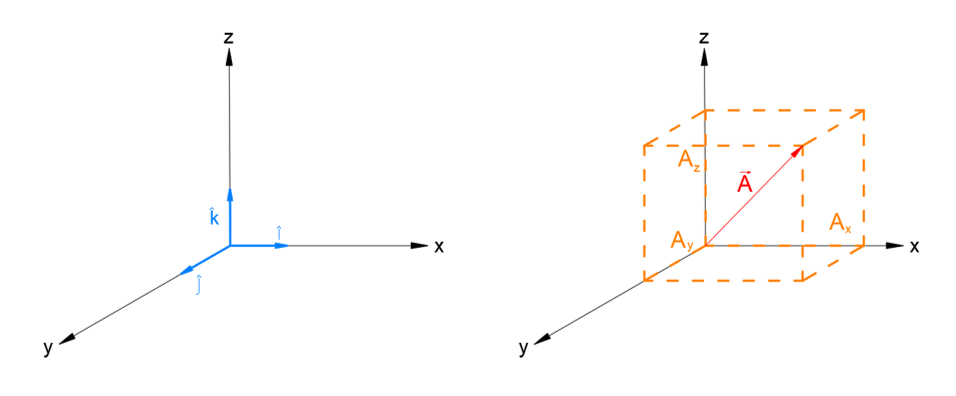
\includegraphics[height=6cm]{Imagenes/vectoreuni.png}
\caption{Representación y suma de vectores}\label{fig:Representacion vectores}
\end{figure}
Además de los vectores también existen los escalares para asignar magnitudes, estos solo poseen magnitud. Los vectores pueden sumarse y restarse, es importante notar que se debe tomar en cuenta la dirección y sentido.\\
El sistema de referencia para ubicar el vector es usualmente el sistema de coordenadas cartesianas, con ejes denotados como $x$, $y$ y $z$. Para mayor facilidad de escritura se asignan vectores unitarios a cada uno de los ejes, siendo $\hat{\imath}$, $\hat{\jmath}$ y $\hat{k}$\\
Ahora denotemos un vetor $\vec{r}\in \mathbb{R}^3$, usando coordenadas cartesianas lo podemos denotar como $\vec{r}=(x,y,z)=x\hat{\imath}+y\hat{\jmath}+z\hat{k}$.\\
Existen operaciones algebraicas posibles con los vectores, estás son:\\
Sea el vector $\vec{A}=(A_x,A_y,A_z)$ y el vector $\vec{B}=(B_x,B_y,B_z)$:
\begin{itemize}
\item Suma de vectores $\vec{A}$ y $\vec{B}$:
$$\vec{A}+\vec{B}=(A_x+B_x)\hat{\imath}+(A_y+B_y)\hat{\jmath}+(A_z+B_z)\hat{k}$$
\item Resta de vectores $\vec{A}$ y $\vec{B}$:
$$\vec{A}-\vec{B}=(A_x-B_x)\hat{\imath}+(A_y-B_y)\hat{\jmath}+(A_z-B_z)\hat{k}$$
\item Mulplicación de un escalar $k$ por un vector $\vec{A}$:
$$k\vec{A}= kA_x \hat{\imath}+kA_y\hat{\jmath}+kA_z\hat{k}$$
\item Producto punto entre vectores $\vec{A}$ y $\vec{B}$:
$$\vec{A} \cdot \vec{B}= A_xB_x+A_yB_y+A_zB_z$$
\item Producto cruz entre vectores $\vec{A}$ y $\vec{B}$:
$$\vec{A} \times \vec{B}= \left| {\begin{array}{ccc}
   \hat{\imath} & \hat{\jmath} & \hat{k} \\
   A_x & A_y & A_z\\
   B_x & B_y & B_z\\
  \end{array} } \right|$$
\end{itemize}
Sea $\Omega$ un espacio abierto en $\mathbb{R}^3$ 
Llamaremos campo vectorial sobre Ω a toda función $$F : Ω ⊆ \mathbb{R}^3\rightarrow\mathbb{R}^3$$
Escribiendo en coordenadas cartesianas esto nos queda:
$$\vec{F}(x,y,z)=\vec{F}_1(x,y,z)\hat{\imath}+\vec{F}_2(x,y,z)\hat{\jmath}+\vec{F}_3(x,y,z)\hat{k}$$
Entonces podríamos definir el campo vectorial como un campo que asocia un vector a cada punto del espacio.
\begin{figure}[H]
\centering
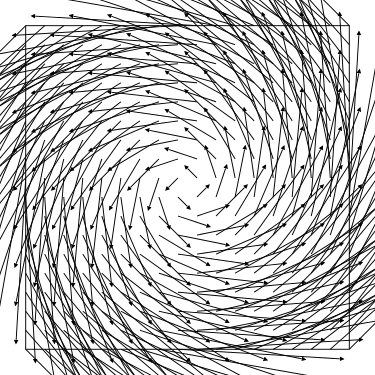
\includegraphics[height=6cm]{Imagenes/campovec.png}
\caption{Campo vectorial. (Fuente: Wikipedia)}\label{fig:Campo vectorial}
\end{figure}
Para graficar estos campos usualmente se escalan los vectores en cada punto de manera que al mirar el campo completo el dibujo sea entendible, es decir escalamos los vectores para que quepan todos en el dibujo. Otra buena manera de graficar estos campos de forma que sean más fácil de interpretar por parte del lector es coloreando las líneas y establecer una escala de colores para poder interpretar de mejor manera.
\begin{figure}[H]
\centering
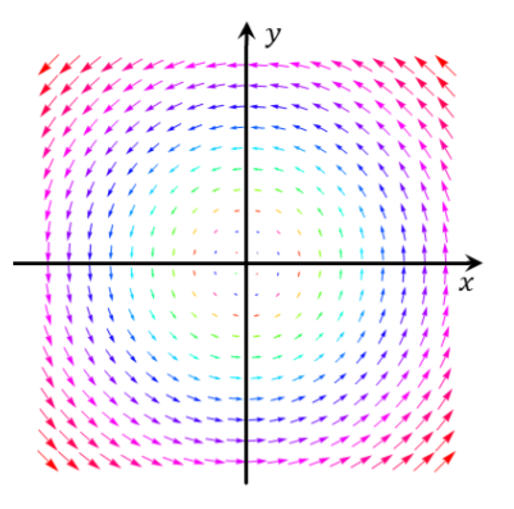
\includegraphics[height=6cm]{Imagenes/campoveccolor.png}
\caption{Campo vectorial. (Fuente: \cite{camposvectoriales})}\label{fig:Campo vectorial en colores}
\end{figure}
Es necesario también saber las operaciones posibles entre campos vectoriales, las fundamentales son 2. El gradiente y el rotacional del campo. Según las definiciones de \cite{camposvectoriales2}:
Sea $f:A\subset \mathbb{R}^3\rightarrow \mathbb{R}^3$ un campo vectorial. Suponiendo las condiciones necesarias de derivación definimos divergencia y rotor respectivamente como:
\begin{equation*} 
\mathnormal{div}\;F(x,y,z)=\frac{\partial F_1}{\partial x}(x,y,z)+\frac{\partial F_2}{\partial y}(x,y,z)+\frac{\partial F_3}{\partial z}(x,y,z)
\end{equation*}
\begin{equation*}
\mathnormal{rot}\;F(x,y,z)=\left(\frac{\partial F_3}{\partial y}-\frac{\partial F_2}{\partial z},\frac{\partial F_1}{\partial z}-\frac{\partial F_3}{\partial x},\frac{\partial F_2}{\partial x}-\frac{\partial F_1}{\partial y}\right)=  \left| {\begin{array}{ccc}
   \hat{\imath} & \hat{\jmath} & \hat{k} \\
   \frac{\partial}{\partial x} & \frac{\partial}{\partial y} & \frac{\partial}{\partial z} \\
   F_1 & F_2 & F_3 \\
  \end{array} } \right|
\end{equation*}
Otro tipo de notación también es utilizada, ocupando el simbolo de gradiente como un operador:
$$\nabla = \left(\frac{\partial}{\partial x},\frac{\partial}{\partial y},\frac{\partial}{\partial z}\right)$$
Entonces, reescribimos la divergencia y el rotor utilizando el producto punto y cruz con nuestro operador de la forma:
$$\nabla \cdot F = \left(\frac{\partial}{\partial x},\frac{\partial}{\partial y},\frac{\partial}{\partial z}\right) \cdot \left(F_1,F_2,F_3\right)=\frac{\partial F_1}{\partial x}+\frac{\partial F_2}{\partial y}+\frac{\partial F_3}{\partial z}=\mathnormal{div}\;F$$
$$\nabla \times F = \left| {\begin{array}{ccc}
   \hat{\imath} & \hat{\jmath} & \hat{k} \\
   \frac{\partial}{\partial x} & \frac{\partial}{\partial y} & \frac{\partial}{\partial z} \\
   F_1 & F_2 & F_3 \\
  \end{array} } \right|
  =\left(\frac{\partial F_3}{\partial y}-\frac{\partial F_2}{\partial z},\frac{\partial F_1}{\partial z}-\frac{\partial F_3}{\partial x},\frac{\partial F_2}{\partial x}-\frac{\partial F_1}{\partial y}\right) = \mathnormal{rot}\;F$$
Este operador se puede aplicar sobre si mismo, este 'nuevo' operador se conoce como el 'operador laplaciano' y corresponde a la divergencia del gradiente, para representarlo se utiliza $\Delta$ o $\nabla^2$:
$$\nabla \cdot (\nabla \cdot F) =\nabla^2 \cdot F =\frac{\partial^2 F_1}{\partial x^2}+\frac{\partial^2 F_2}{\partial y^2}+\frac{\partial^2 F_3}{\partial z^2}$$
Existen dos propiedades importantes que debemos tener en cuenta:
\begin{equation}
\label{eq:Rotor de una divergencia}
\nabla \times (\nabla \cdot F)=0
\end{equation}

\begin{equation}
\label{eq:Identidad gradiente}
\nabla \cdot (fV)=f\cdot (\nabla V)-V\cdot\nabla f
\end{equation}
Otro concepto de cálculo vectorial que debemos tener claro son los campos vectoriales conservativos los cuales son de vital importancia en el campo físico. 
Los campos vectoriales que pueden ser definidos bajo el gradiente de una función escalar $f$ son llamados conservativos. Esto es $\vec{F}=\vec{\nabla} f$, además la función escalar $f$ es conocida como la función potencial del campo $\vec{F}$.\\
En otras palabras, esto es, siendo el campo vectorial $\vec{F}(x,y,z)=\vec{F}_1(x,y,z)\hat{\imath}+\vec{F}_2(x,y,z)\hat{\jmath}+\vec{F}_3(x,y,z)\hat{k}$ la función potencial $f(x,y,z)$ del campo $\vec{F}$ está definida como:
$$\frac{\partial f}{\partial x}(x,y,z)=F_1(x,y,z),\qquad \frac{\partial f}{\partial y}(x,y,z)=F_2(x,y,z),\qquad \frac{\partial f}{\partial z}(x,y,z)=F_3(x,y,z)$$
\section{Cálculo integral.}\label{sec:Calculo integral.}
\setcounter{figure}{0}
\setcounter{equation}{0}
En BEM resolveremos ecuaciones diferenciales, en donde a las funciones diferenciales se les aplica muchas veces el concepto de integral. Si bien en este documento no nos adentraremos en demasía en el tema, los teoremas que se presentan a continuación serán de gran utilidad para resolver la problematica planteada:
\begin{itemize}
\item Teorema fundamental del cálculo: Sea $f$ una función escalar.
\begin{equation}
\label{eq:Teorema fundamental del calculo}
\int^b_a \frac{df(x)}{dx}dx=f(b)-f(a)
\end{equation}
\item Teorema fundamental del gradiente: Sea $F$ una función vectorial.
\begin{equation}
\label{eq:Teorema fundamental del gradiente}
\int^b_a \nabla F ds=F(b)-F(a)
\end{equation}
\item Teorema de Gauss:
\begin{equation}
\label{eq:Teorema de Gauss}
\int_\Omega(\nabla\cdot F)d\Omega=\oint_\Gamma n\cdot F d\Gamma
\end{equation}
\item Integración por partes:
\begin{equation}
\label{eq:Integracion por partes}
\int u dv=uv-\int v du
\end{equation}
\end{itemize}

\section{Campo eléctrico y campo magnético.}\label{sec:Campo electrico y campo magnetico.}
\setcounter{equation}{0}
\setcounter{figure}{0}
Es importante tener claros los conceptos de campo eléctrico y campo magnético antes de adentrarnos en el problema. En esta sección veremos la definición de ambos campos, sus propiedades y un esquema ilustrativo, para ayudar a entender de mejor manera estas ideas.
\subsection{Campo eléctrico.}
Como definición el campo eléctrico es 'Campo físico que describe la interaccón entre 2 cuerpos o sistemas con propiedades de naturaleza eléctrica'. Está representado por la letra $E$, también se podría definir como la fuerza eléctrica $F_{e}$  por unidad de carga $q$ o bien:
$$E=\frac{F}{q}$$
El campo eléctrico estático puede representarse esquemáticamente a tráves de líneas, conocidas como \textbf{líneas de campo}.
\begin{figure}[H]
\centering
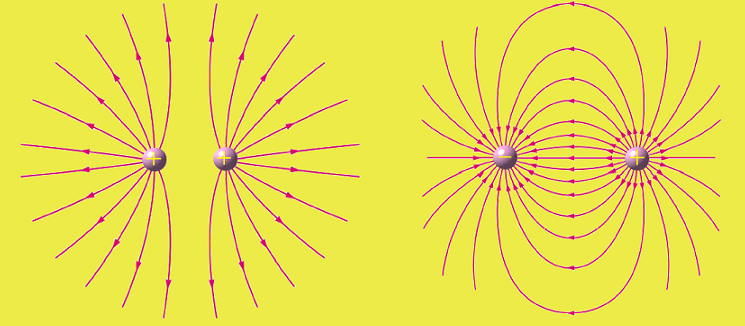
\includegraphics[height=6.8cm]{Imagenes/Lineas_de_campo.png}
\caption{Líneas de campo eléctrico}\label{fig:Lineas de campo electrico}
\end{figure}
Las líneas de campo eléctrico poseen las siguientes carácteristicas:
\begin{itemize}
\item El vector de campo eléctrico en cualquier punto es tangente a la línea que pasa por dicho punto.
\item Las líneas de campo no se cruzan.
\item El número de líneas que salen de una carga positiva o entran en una carga negativa es proporcional a dicha carga.
\item Las líneas de campo no pueden cortarse. De lo contrario en el punto de corte existirían dos vectores campo eléctrico distintos.
\item A grandes distancias de un sistema de cargas, las líneas están igualmente espaciadas y son radiales, comportándose el sistema como una carga puntual.
\end{itemize}
\subsection{Campo magnético.}
El campo mágnetico, al igual que el campo eléctrico es una magnitud vectorial. Es generado por cargas en movimiento, estas pueden ser puntuales o un conjunto de cargas o en otras palabras, una corriente eléctrica. Su unidad de medida es el tesla $(T)$.\\
El movimiento de una carga puntual produce un campo magnético de la forma:
\begin{figure}[H]
\caption{Campo magnético por una carga puntual.}
\centering
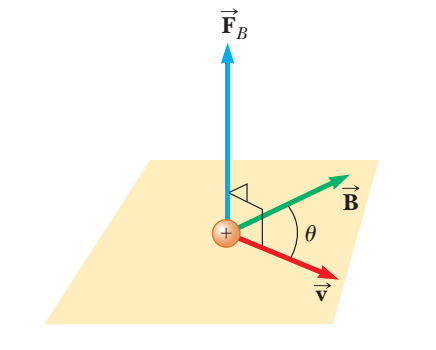
\includegraphics[height=4cm]{Imagenes/campomag.png}\label{fig:Campo magnetico}
\end{figure}
El campo magnético viene dado por:
$$\overrightarrow{B}=\frac{\mu_0}{4\pi}\,\frac{q\,\overrightarrow{v}\times\overrightarrow{u_r}}{r^2}$$
Donde $q$ es la carga puntual que crea el campo, $v$ es la velocidad de $q$, $r$ es la distancia desde $q$ hasta $P$, $P$ es el punto donde estamos calculando el campo magnético, $u_r$ es un vector unitario que va desde $q$ hasta $P$, $μ_0$ es una constante denominada permeabilidad del espacio libre. Su valor en el Sistema Internacional es $μ_0 = 4 \pi 10^{-7} T m/A$.\\
Por otro lado, una corriente eléctrica son muchas cargas puntuales moviendose en conjunto, por lo que también generan un campo magnético. En este caso el calculo del campo será con elementos infinitesimales:
\begin{figure}[H]
\caption{Campo magnético por una corriente eléctrica.}
\centering
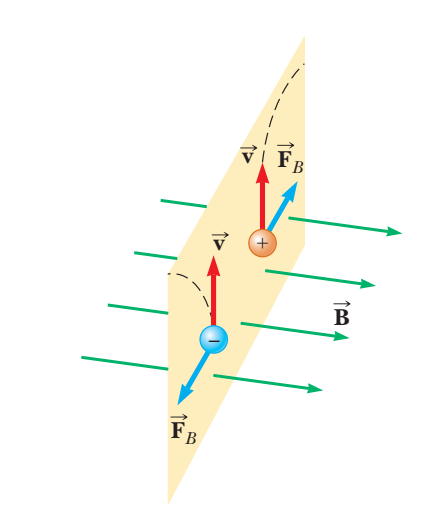
\includegraphics[height=4cm]{Imagenes/campomag_corr.png}\label{fig:Campo magnetico por una corriente}
\end{figure}
En donde $I$ es la intensidad de la corriente, dada por la fórmula $I=q\,n\,v_d\,A$, con $n$ siendo la cantidad de cargas, $A$ la sección del hilo y $v_d$ la velocidad del desplazamiento.
$$d\overrightarrow{B}=\frac{μ_0}{4\pi}\, \frac{I\,\overrightarrow{dl}\times \overrightarrow{u_r}}{r^2} $$
\subsection{Leyes de Maxwell.}\label{sec:Leyes de Maxwell}
Como vimos anteriormente existen campos eléctricos y campos magnéticos, el conjunto de ambos campos se conoce como campo electromagnético. A tráves de este campo, los elementos que interactúan entre si por medio de la electricidad o el magnetismo se comportan siguiendo ciertas reglas de como los elementos perturban al campo, o como el campo se perturba a si mismo. Estas reglas son conocidas como las ecuaciones o leyes de Maxwell.\\
En un principio eran 8, luego se condensaron en 4 y se pueden escribir como: 
\begin{equation}
\label{eq:maxwell1}
\vec {\nabla} \cdot\vec{E}=\frac{\rho}{\varepsilon_0}\\
\end{equation}
\begin{equation}
\label{eq:maxwell2}
\vec {\nabla} \cdot\vec{B}=0\\
\end{equation}
\begin{equation}
\label{eq:maxwell3}
\vec {\nabla} \times\vec{E}=-\frac{\partial \vec{B}}{\partial t}\\
\end{equation}
\begin{equation}
\label{eq:maxwell4}
\vec {\nabla} \times\vec{B}=\mu_0\vec{J}+\mu_0\varepsilon_0\frac{\partial \vec{E}}{\partial t}\\
\end{equation}
Para entender un poco más las ecuaciones, pasaremos a explicaralas. La ecuación \eqref{eq:maxwell1} también conocida como la \textbf{Ley de Gauss} nos dice básicamente que las cargas positivas serán fuentes y que las cargas negativas serán sumideros, tal cual como se ve en la imagen \ref{fig:Lineas de campo electrico}, en otras palabras, cargas del mismo signo repelen y cargas opuestas se atraen, notar que $\rho$ es la densidad de carga y $\varepsilon_0$ es la permitividad eléctrica en el vacío. Esta ley también nos indica que el campo eléctrico decae con la distancia, lo hace a razón de $1/r^2$. La ecuación \eqref{eq:maxwell2}, algo así como la Ley de Gauss del magnetismo, indica que no hay fuentes o sumideros de campo magnético, lo que no impide que hayan elementos que generen campos magneticos, como vimos anteriormente. ¿Por qué es importante esto? Porque nos indica que el campo magnético siempre debe cerrarse sobre si mismo. De forma práctica esto se ve al cortar un imán por la mitad, si bien en un inicio solo existe un polo sur y otro norte, al cortarlo en 2 cada trozo tiene su polo sur y norte respectivamente. Es decir, los monopolos no existen. La ecuación \eqref{eq:maxwell3}, también conocida como la \textbf{Ley de Faraday}  nos dice que si un campo magético cambia en el tiempo este 'activa' el campo eléctrico, por lo tanto no solo las cargas e imanes influyen en los campos sino que estos influyen entre si, lo que nos lleva directamente a la ecuación \eqref{eq:maxwell4} o la \textbf{Ley de Ampère-Maxwell} que también nos dice que si el campo eléctrico cambia en el tiempo o cargas moviendose, es decir una corriente eléctrica denotada en la ecuación como $\vec{J}$, esto activará el campo magnético. Las constantes utilizadas en las ecuaciones son:
\begin{itemize}
\item Permitividad eléctrica en el vacío
$$\varepsilon_0=8.85\times 10^{-12} \left[\frac{C^2}{N\cdot m^2}\right]$$
\item Permisividad magnética en el vacío
$$\mu_0=4 \pi \times 10^{-7}\left[\frac{N}{A^2}\right]$$
\end{itemize}

Combinando estas 4 leyes es válido decir que todos los fenómenos electromagnéticos que percibimos se pueden explicar. 
\begin{figure}[H]
\caption{Líneas de campo magnético.}
\centering
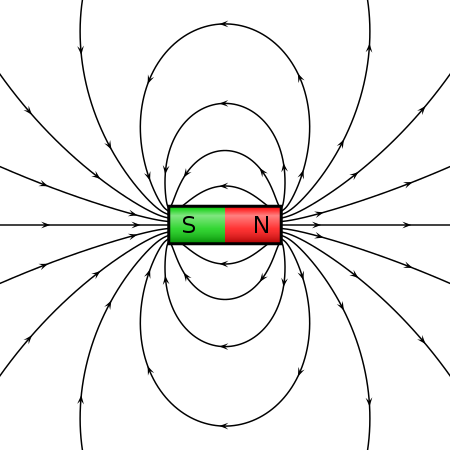
\includegraphics[height=5.5cm]{Imagenes/lineasmag.png}\label{fig:Lineas de campo magnetico}
\end{figure}
Las ecuaciones descritas con anterioridad son dadas para el medio vacío. Para el caso en que los elementos se encuentre en un medio es necesario adaptar las propiedades del mismo. Se pueden encontrar una nueva relación para $E$ y $B$ a través de dos parámetros ya conocidos, como permitividad eléctrica y permisividad magnética. La relación es de la forma:
$$\vec{E}=\frac{\vec{D}}{\varepsilon}$$
$$\vec{B}=\mu \vec{H}$$
En donde $D$ se define como la densidad el flujo eléctrico y $H$ como la intensidad del campo magnético. Se dice que si la relación entre  $E/D$ y $B/H$ estamos en presencia de un medio lineal. Esto permite que $\varepsilon$ y $\mu$ se representen de forma matricial. Si esta matriz se puede diagonalizar, es decir que que solo existan en la diagonal se habla de un medio isótropo y si además los elementos no son iguales se habla de un medio anisótropo. Un elemento isótropo es un elemento en el que sus cualidades físicas no dependen de la dirección en la que son examinadas, por el contrario en el anisótropo su dirección varía sus propiedades físicas.
\section{Ecuaciónes Diferenciales.}\label{sec:Ecuaciones Diferenciales.}

En este documento investigaremos el comportamiento de dos ecuaciones de gran importancia en el modelamiento físico de varios fenómenos, por lo que es necesario tener un poco de entendimiento sobre su comportamiento matemático.
\subsection{Ecuación de Laplace.}
Esta es una ecuación de derivadas parciales de tipo elíptico. Es un caso particular de la ecuación de Helmholtz, sin embargo, la ecuación de Laplace junto con la ecuación de Poisson son los dos modelos más simples de las ecuaciones en derivadas parciales (EDP) de tipo elípticas.\\
La ecuación de Laplace en se puede escribir de distintas formas:
Escrita con el operador nabla $\nabla$
\begin{equation}
\nabla^2\phi=0
\end{equation}
Escrita en derivadas, para el caso tridimensional, en coordenadas cartesianas:
\begin{equation}
\frac{\partial^2 \phi}{\partial x^2}+\frac{\partial^2 \phi}{\partial y^2}+\frac{\partial^2 \phi}{\partial z^2}=0
\end{equation}
Esta ecuación es la encargada de modelar el comportamiento de, por ejemplo, el potencial eléctrico en una región sin cargas.
\subsection{Ecuación de Helmholtz.}
Esta ecuación, por otro lado, está compuesta por:
\begin{equation}
(\nabla^2+k^2)\phi=0
\end{equation}
\newpage
\section{Método de elementos de borde.}\label{sec:BEM.}
\setcounter{figure}{0}
\setcounter{equation}{0}
El método de elementos de borde o BEM por sus siglas en inglés Boundary Element Method, es en escencia un método númerico para la resolución de ecuaciónes diferenciales, es muy utilizado en mecánica de fluidos, acústica, electromagnética, entre otras áreas. Cuando leemos esta definición es inevitable pensar en el método de elementos finitos o FEM, el cúal es el modelo más clasico de la resolución de este tipo de ecuaciones, pero ¿en qué se diferencian?\\
Como bien sabemos, las ecuaciones diferenciales rigen una gran cantidad de fenómenos físicos. Para resolver estas ecuaciones diferenciales se realiza un proceso llamado discretización, el cual nos entrega resultados aproximados y consiste en dividir el elemento en estudio en elementos infinitesimales y basandose en las expansiones de Taylor, poder encontrar el resultado buscado. Es aquí justamente donde encontramos la primera gran diferencia entre ambos métodos:
\begin{figure}[H]
\centering
\label{fig:Discretizacion BEM y FEM}
\subfigure[Discretización utilizada en BEM.]{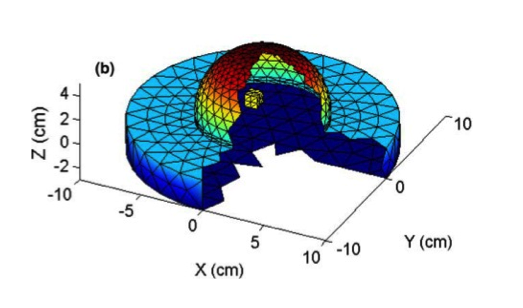
\includegraphics[height=6.8cm]{Imagenes/DiscretizacionBEM.png}}
\subfigure[Discretización utilizada en FEM.]{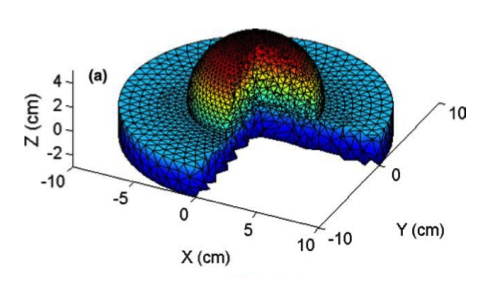
\includegraphics[height=6.8cm]{Imagenes/DiscretizacionFEM.png}}
\caption{Diferencias en la discretización en BEM y FEM en 3D.}
\end{figure}
Como observamos en la imagen, el elemento infinitesimal de estudio en FEM es un pequeño elemento de 3 dimensiones, puede ser un cubo, una piramide. Mientras que en BEM, el elemento es en 2D, triángulos, cuadrados, etc. Cabe destacar que mientras más elementos se utilicen para dividir el objeto de estudio, más preciso será el cálculo.\\
El BEM utiliza condiciones de borde o de frontera para ajustar los valores de borde a las ecuaciones diferenciales. Estás condiciones suelen ser:
\begin{equation}
\label{eq:Condiciones iniciales}
\begin{split}
\textnormal{Condiciones 'esenciales' del tipo }u=\bar{u}\textnormal{ en }\Gamma_1\\
\textnormal{Condiciones 'naturales' del tipo }q=\bar{q}\textnormal{ en }\Gamma_2
\end{split}
\end{equation}
Estas condiciones usualmente son conocidas como condiciones de Dirichlet, las condiciones 'esenciales', mientras que las condiciones 'naturales' son conocidas como condiciones de Neumann. Pueden existir condiciones de frontera más complejas tal como la combinación de las dos anteriores.\\
La ecuación integral que se usa como punto de inicio para el método es:
\begin{equation}
\label{eq:Ecuacion inicial BEM}
\nabla^2u=0
\end{equation}
Si a esta ecuación se le aplica una integral por el volumen $\Omega$ y además se multiplica por una función $w$ conveniente:
\begin{equation}
\int_\Omega\nabla^2u(r')w(r-r')\;d\Omega(r')=0
\end{equation}
Notar que estamos integrando sobre $r'$ y $r$ no está restringida. Utilizando la identidad mostrada en la ecuación \eqref{eq:Identidad gradiente} se puede descomponer de la forma :
\begin{equation}
\label{eq:Descomposicion 1}
\int_\Omega w(r-r')\nabla\cdot(\nabla u(r'))\;d\Omega(r')=\int_\Omega\nabla\cdot u(r')(\nabla w(r-r'))\;d\Omega(r')-\int_\Omega\nabla u(r')\nabla w(r-r')\;d\Omega(r')
\end{equation}
En el primer término del lado derecho de la ecuación \eqref{eq:Descomposicion 1} podemos utilizar el teorema de Gauss, indicado en la ecuación \eqref{eq:Teorema de Gauss}, mientras que en el segundo término volvemos a utilizar la identidad \eqref{eq:Identidad gradiente}, lo que nos entrega\footnote{Para facilidad de notación solo se utilizará $u$ y $w$}:
\begin{equation}
\int_\Omega \nabla^2u\;w\;d\Omega=\int_\Gamma n\cdot u\nabla w\;d\Gamma-\int_\Omega\nabla\cdot(w\nabla u)d\Omega-\int_\Omega v\nabla\cdot\nabla u\;d\Omega
\end{equation}
\begin{figure}[H]

\centering
\subfigure[Hemisfera alrededor de $i$]{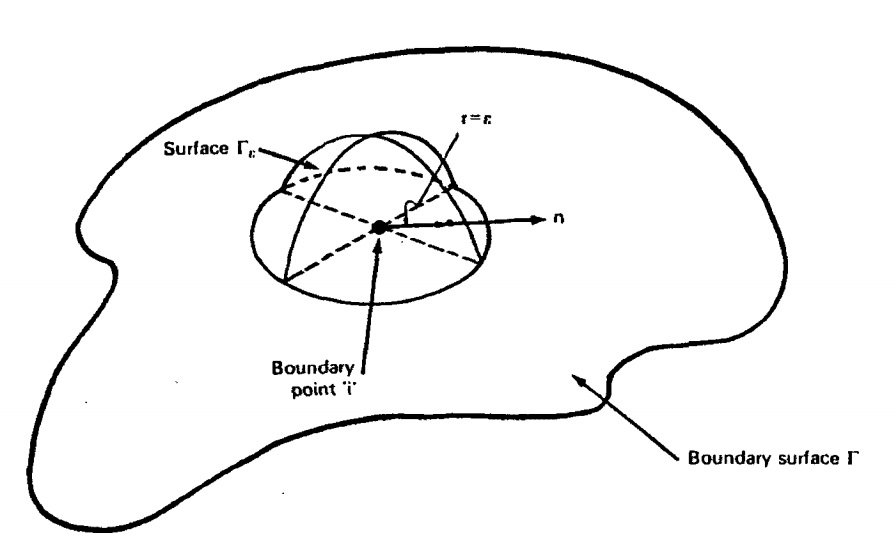
\includegraphics[scale=0.35]{Imagenes/2.2.jpg}}
\subfigure[Semicirulo alrededor de $i$]{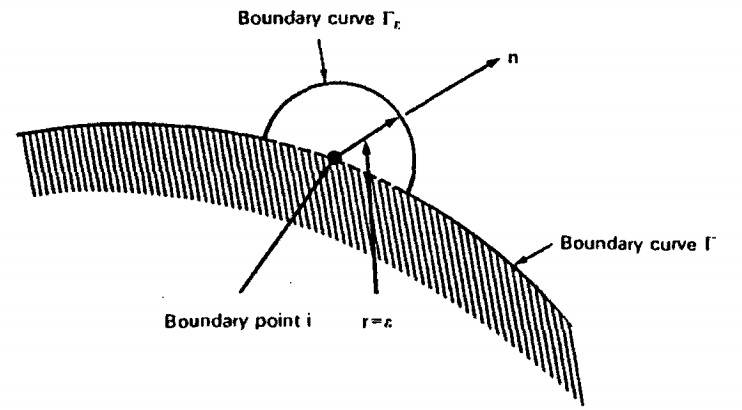
\includegraphics[scale=0.35]{Imagenes/2.3.jpg}}
\caption{Puntos de frontera para los casos 2D y 3D (Fuente:\cite{Brebbia})}\label{fig:Singularidades}
\end{figure}
Nuevamente podemos utilizar el teorema de Gauss con el segundo término del lado derecho de la ecuación. Además, igualamos la ecuación a cero tal como en \eqref{eq:Ecuacion inicial BEM}:
\begin{equation}
0=\int_\Gamma n\cdot u\nabla w\;d\Gamma-\int_\Gamma n\cdot w\nabla u\;d\Gamma-\int_\Omega u \nabla^2 w\;d\Omega
\end{equation}
Ahora llamaremos a nuestra función $w$ conveniente la solución fundamental de la ecuación, la cual tiene por segunda dervada la función Delta Dirac, la que si se encuentra bajo el dominio de la solución de la función tiene por valor 1, como este es el caso se puede afirmar que el tercer término de la ecuación tiene por valor $u(r)$. Sin embargo también hay que recordar que la función $w$ está evaluada en $(r-r')$ por lo que hay una singularidad que ocurre cuando $r\rightarrow r'$ que se debe estudiar. Esta singularidad, que está ilustrada en la figura \ref{fig:Singularidades}, genera un término libre de valor $-1/2\;u(r)$. Finalmente podemos escribir la ecuación como:
\begin{equation}
0=\int_\Gamma n\cdot u\nabla w\;d\Gamma-\int_\Gamma n\cdot w\nabla u\;d\Gamma+\frac{1}{2}u
\end{equation}
Tomando como nueva notación a $w=u*$. Notar que las divergencias están multiplicadas por un vector normal, por lo que el término afectado por el operador $\nabla$ se transforma en la derivada en la dirección normal. Reescribiendo llegamos a:
\begin{equation}
\label{eq:Ecuacion inicial BEM desarrollada}
\frac{1}{2}u^i+\int_\Gamma uq^*\,d\Gamma=\int_\Gamma qu^*\,d\Gamma
\end{equation}
En donde $u$ es una función potencial, $q$ es su derivada con respecto a la normal. $u^*$ y $q^*$ son las soluciones fundamentales de ambas funciones. El superindice $i$ indica el punto de 'anclaje' o centro del círculo o hemiesfera de interés.
Estos puntos $i$ serán considerados como 'nodos'. 
Al momento de discretizar la ecuación \eqref{eq:Ecuacion inicial BEM desarrollada} nos queda de la siguiente forma:
\begin{equation}
\label{eq:Ecuacion discretizada}
\frac{1}{2}u^i+\sum_{j=1}^N\left( \int_{\Gamma_j} q^*\,d\Gamma\right)u^j=\sum_{j=1}^N \left(\int_{\Gamma_j} u^*\,d\Gamma \right)q^j
\end{equation}
Las integrales mostadas, se llamarán para simplificar:
\begin{equation}
\label{eq:Descripcion de matriz H y G}
\hat{H}^{ij}=\int_{\Gamma_j}q^*\,d\Gamma\qquad\textnormal{ y }\qquad G^{ij}=\int_{\Gamma_j}u^*\,d\Gamma
\end{equation}	 
\begin{figure}[H]
\label{fig:Tipo de elemento de frontera}
\centering
\subfigure[Elementos constantes.]{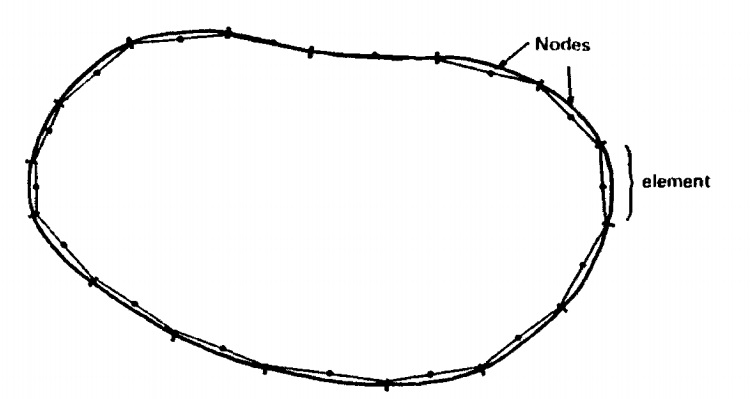
\includegraphics[scale=0.35]{Imagenes/elementos constantes.jpg}}
\subfigure[Elementos lineales.]{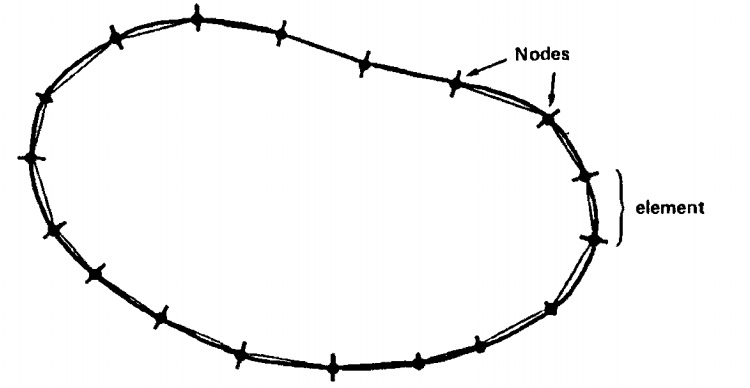
\includegraphics[scale=0.35]{Imagenes/elementos lineales.jpg}}
\subfigure[Elementos cuadráticos.]{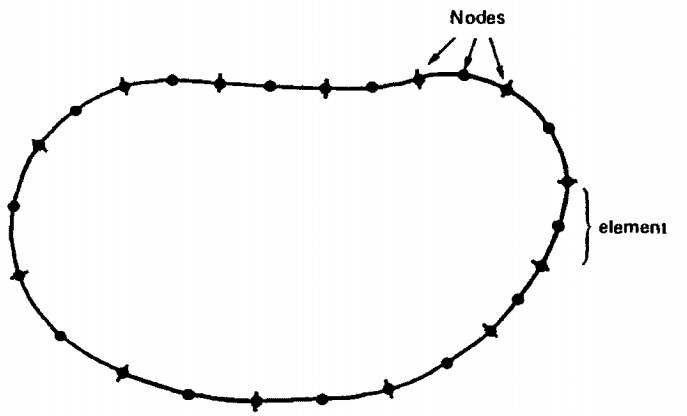
\includegraphics[scale=0.35]{Imagenes/elementos cuadraticos.jpg}}
\caption{Diferentes tipos de elementos de frontera. (Fuente:\cite{Brebbia})}
\end{figure}
\begin{equation*}
\label{eq:Desarrollo de H}
\left.
\begin{aligned}
\textnormal{Si }i\not = j&\textnormal{ entonces } \hat{H}^{ij}\\
\textnormal{Si }i\not = j&\textnormal{ entonces } \hat{H}^{ij}+\frac{1}{2}
\end{aligned}
\right\}
=H^{ij}
\end{equation*}
Entonces la ecuación \eqref{eq:Ecuacion discretizada} puede ser escrita como:
\begin{equation}
\label{eq:Sumatoria de H y G}
\sum_{j=1}^NH^{ij}u^j=\sum_{j=1}^N G^{ij}q^j
\end{equation}
Esta serie de ecuaciones puede ser expresada en forma de matriz como:
\begin{equation}
\label{eq:Forma matricial HU=GQ}
HU=GQ
\end{equation}
Podemos llevar todos los términos conocidos al lado izquierdo y los valores iniciales conocidos (como los ejemplificados en la ecuación \eqref{eq:Condiciones iniciales}), reescribiendola como:
\begin{equation}
\label{eq:Forma matricial AX=F}
AX=F
\end{equation}
Entonces, si nuestras condiciones iniciales son solo de Dirichlet, el vector $X$ estaría compuesto solo por 'valores desconocidos' de $q$ y viceversa. Si fuera una mezcla de ambas condiciones, el vector $X$ sería una mezcla de $u's$ y $q's$, evidentemente luego deberían reordenarse los valores y dejar un solo vector de $u's$ y otro distinto para $q's$. Esto es consecuencia de la formulación mixta de elementos de frontera y entrega una importante ventada respecto a elementos finitos.
\begin{figure}[H]
\label{fig:Discretizacion BEM y FEM 2}
\centering
\subfigure[Discretización utilizada en BEM.]{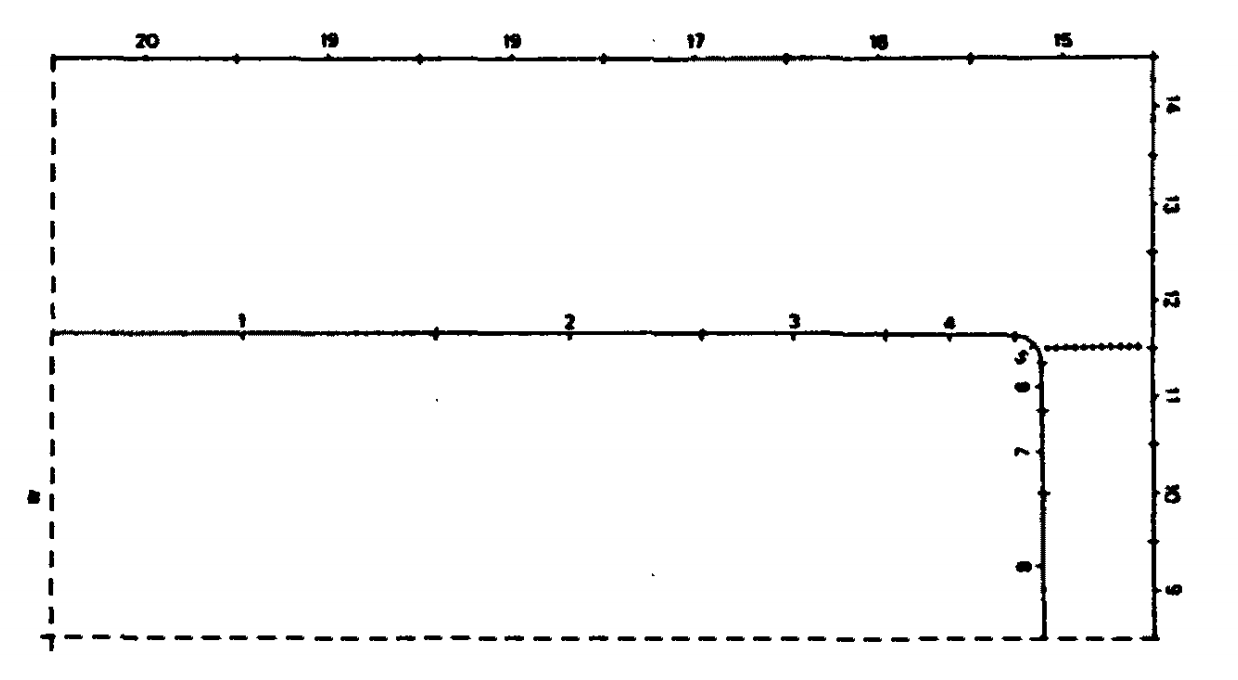
\includegraphics[height=6.8cm]{Imagenes/disbem.png}}
\subfigure[Discretización utilizada en FEM.]{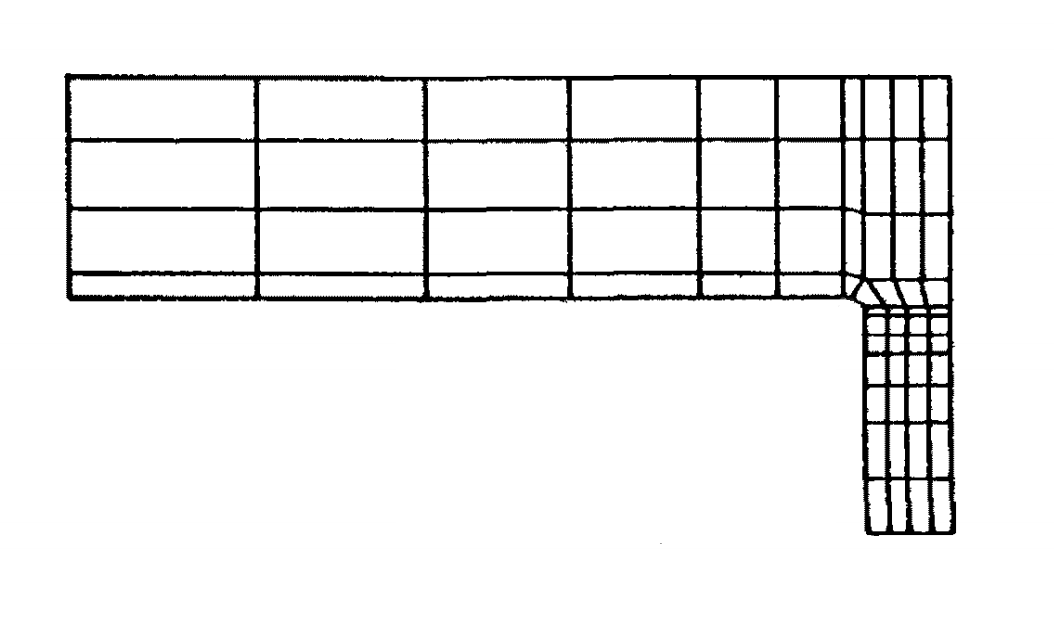
\includegraphics[height=6.8cm]{Imagenes/disfem.png}}
\caption{Diferencias en la discretización en BEM y FEM en 2D  (Fuente:\cite{Brebbia}).}
\end{figure}
Es necesario hacer un par de alcances, para comprender mejor lo explicado anteriormente:
Las integrales mostradas en la ecuación \eqref{eq:Descripcion de matriz H y G} son resueltas mediante una cuadratura de Gauss, la cual es una aproximación de la integral. En el problema a resolver en este informe, se utiliza una cuadratura con 4 nodos.\\
Es importante indicar que BEM es aplicable a problemas que puedan ser modelados por una función de Green, ya sea Laplace, Helmholtz o Helmholtz modificado. Es necesario hacer notar que las funciones de Green son principalmente utilizadas para modelar ecuaciones diferenciales con condiciones de contorno dadas, que es justamente como hemos definido los problemas de BEM.
\newpage
¿Qué sucede con los puntos internos? Como dijimos en un principio, el comportamiento en el interior del cuerpo de estudio es homogeneo, por lo tanto es posible hacer una buena aproximación o predicción de como se comportará la función potencial estudiada en el cuerpo en los puntos interiores. Gráficamente los puntos interiores serían algo como:
\begin{figure}[H]
\centering
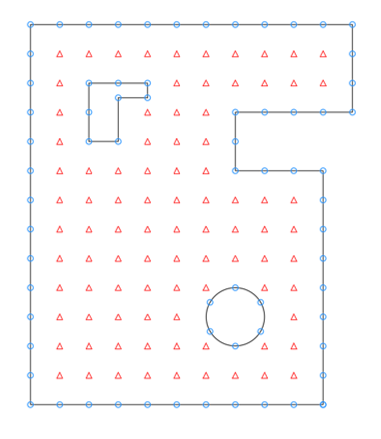
\includegraphics[scale=1]{Imagenes/bem.png}
\caption{Elementos de borde y puntos internos para el estudio}\label{fig:Puntos internos de BEM}
\end{figure}
Para calcular el potencial es necesario utilizar la ecuación que se muestra a continuación. Es necesario hacer notar que los coeficientes $H^{ij}$ y $G^{ij}$ son recalculados para cada punto interno. 
\begin{equation}
\label{eq:Calculo puntos internos discretizada}
u^i=\sum_{j=1}^NG^{ij}q^j-\sum_{j=1}^N\hat{H}^{ij}u^j
\end{equation}
El cálculo para la derivada en ambas direcciones en los puntos internos también se puede realizar, pero su formulación es como sigue:
\begin{equation}
\label{eq:Calculo derivada en puntos internos}
\begin{split}
\left(q_{x_1}\right)=\left(\frac{\partial u}{\partial x_1}\right)^i=\sum_{j=1}^N\left(\int_\Gamma \frac{\partial u^*}{\partial x_1}\,d\Gamma\right)q^j-\sum_{j=1}^N\left(\int_\Gamma \frac{\partial q^*}{\partial x_1}\,d\Gamma\right)u^j\\
\left(q_{x_2}\right)=\left(\frac{\partial u}{\partial x_2}\right)^i=\sum_{j=1}^N\left(\int_\Gamma \frac{\partial u^*}{\partial x_2}\,d\Gamma\right)q^j-\sum_{j=1}^N\left(\int_\Gamma \frac{\partial q^*}{\partial x_2}\,d\Gamma\right)u^j\\
\end{split}
\end{equation}
\newpage
\section{Biblioteca bempp.}\label{sec:Biblioteca bempp.}
\setcounter{figure}{0}
\setcounter{equation}{0}
Bempp es una plataforma computacional gratuita de elementos de frontera se puede utilizar para resolver problemas de acústica o electroestática, entre otros. Utiliza una interfaz de python de fácil uso, en nuestro caso utilizamos $Docker$\footnote{Software que crea contenedores virtuales para que puedan ejecutarse bajo cualquier máquina, independiente del sistema operativo que tenga.} $Images$ para poder resolver nuestro problema.\\ 
Como se vio en la sección anterior, para resolver problemas con BEM es necesario resolver sistemas compuestos por matrices de gran tamaño, las cuales a su vez contienen elementos que son necesario aproximar, es por esto que la existencia de esta libreria abierta facilita la tarea.
\subsection{Estructura.}
La librería bempp tiene una estructura basada en la imagen \ref{fig:Estructura BEM}, la cual tiene 5 grandes ejes y es explicado con mayor detalle en \cite{Solvingbempp}:
\begin{itemize}
\item Grid: Responsable del manejo de la malla, apoyado en la librería 'Dune-FoamGrid'.
\item Fiber (\textbf{F}ast \textbf{I}ntegration \textbf{B}oundary \textbf{E}lement \textbf{R}outine): Es un elemento vital dentro de la librería. Encargado de evaluaciones las integrales de elementos de borde en cada elemento, sin importar su conectividad. Además de realizar la integración como tal. Este modulo es independiente del resto por lo que podría ser utilizado de manera particular en otros códigos de BEM.
\item Space: Responsable del espacio de funciones y sus derivadas. También actúa como administrador de grados de libertad, usando los conocimientos de la conectividad entre elementos y las propiedades de continuidad del espacio de funciones.
\begin{figure}[H]
\centering
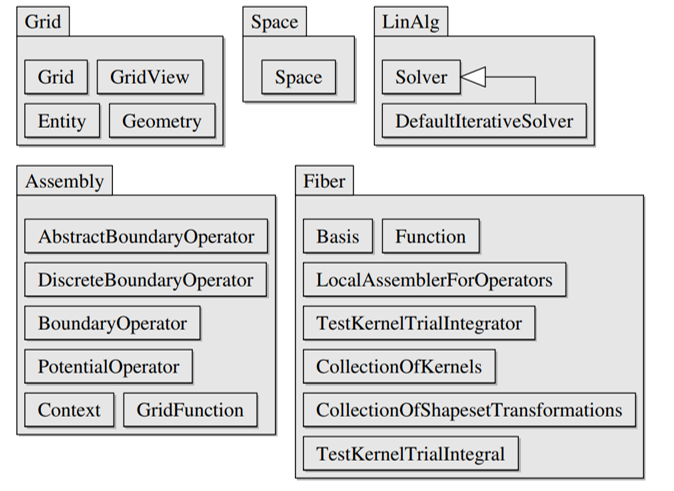
\includegraphics[scale=0.7]{Imagenes/estructurabempp.png}
\caption{Modulos de bempp (Fuente:\cite{Solvingbempp})}\label{fig:Estructura BEM}
\end{figure}
\item Assembly: Es el modulo más grande de la librería. Define los operadores integrales y los espaciones de funciones en la malla. También almacena las matrices de las integrales discretizadas que son formadas en el módulo Fiber.
\item LinAlg: Módulo que almacena distintos tipos de $solver$'s lineales. 
\end{itemize} 


\subsection{Algoritmo y explicación.}
Antes de comenzar a desmenuzar la resolución del problema o el código utilizado es más importante definir que es \textbf{bempp}\cite{bempp}.\\
 El algoritmo para la resolución de problemas a través de bempp es más bien simple pero es necesario tener los conceptos claros o no podremos ejecutarlo de forma correcta. La forma de resolución es la que se muestra a continuación. Es necesario indicar que esta resolución resolvera los parametros de borde, para resolver los elementos internos simplemente se debe realizar una nueva malla con puntos internos y utilizar la solución calculada.
 \begin{figure}[H]
 \centering
 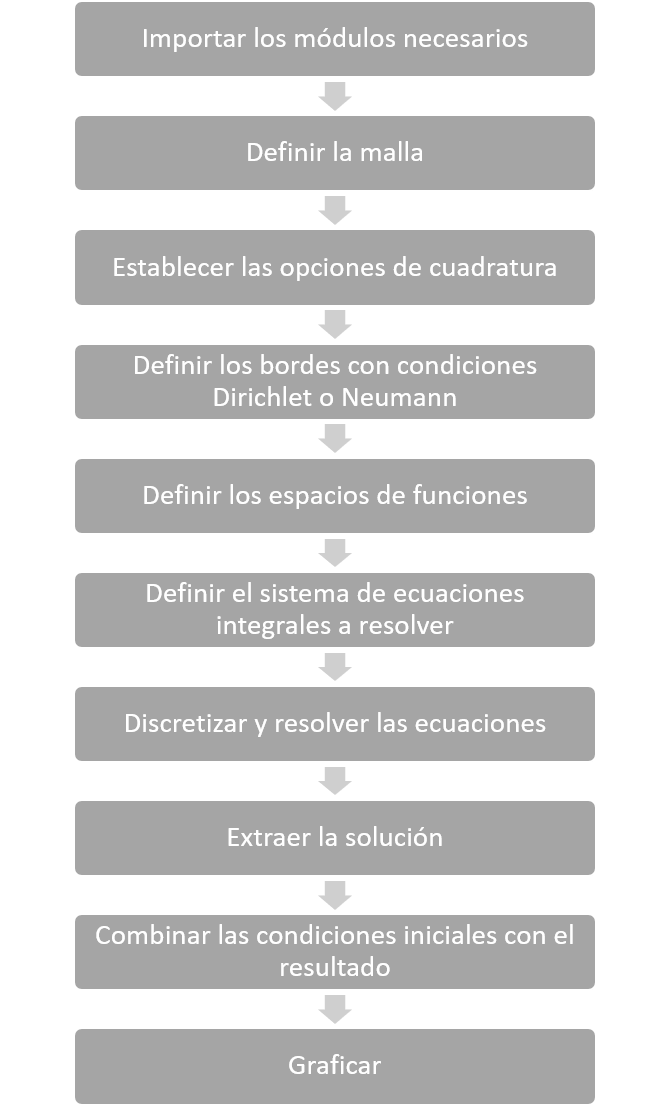
\includegraphics[scale=0.75]{Imagenes/Algoritmo bempp.png}
 \caption{Algoritmo resolución bempp}\label{fig:Algoritmo de BEM}
 \end{figure}

Al observar el esquema se nos hace evidente definir los conceptos y además mostrar como se ejecutó lo descrito en el código:
\begin{enumerate}
\item \textbf{Importar los módulos necesarios.}\\
Módulos: También conocidas como bibliotecas o librerías, añaden funciones adicionales a nuestro lenguaje de programación de uso: Python. Para resolver el problema se utilizaron 3: numpy, scipy.sparse.linalg (para resolver sistemas lineales) y por supuesto, bempp.
\item \textbf{Definir la malla.}\\Malla - Grid: El mallado en esta plataforma puede realizarse de manera bastante simple, siempre y cuando la figura sea común (esferas, cubos, etc...). Estas también pueden ser importadas desde el formato Gmsh.
\item \textbf{Establecer las opciones de cuadratura.}\\Cuadratura - Quadrature: Como vimos en el código manual, hay que utilizar una cuadratura Gaussiana para resolver las ecuaciones integrales, en este punto se precisa de cuantos puntos se hará esa cuadratura. Para asimilar esta forma de resolución lo más posible a la anterior utilizaremos nuevamente 4 puntos.
\item \textbf{Definir los espacios de funciones.}\\Conocido como espacio de función o Function spaces. Como sabemos los nodos podían ser tomados para medios constantes, lineales o polinomiales, dependiendo del medio en que queramos definir nuestros nodos, nuestros espacios de función deben ser definidos en el orden deseado. En la plataforma bempp es importante definir esto correctamente. Como se señala en el algortimo es necesario haber generado con anterioridad la malla, ya que esto es un input necesario. Los tipos de 'Function spaces' que nos interesan son escalares y son utilizados para resolver problemas de Laplace y Helmholtz:
\begin{itemize}
\item \textbf{Continuos Polynomial "P": } Se refiera a que el 'espacio' entre nodos debe tener continuidad, a modo de ejemplo se tiene la figura \ref{fig:Interseccion elementos continuos} la cual nos muestra una intersección de elementos lineales continuos. Este espacio no puede utilizarse con elementos constantes ya que todos deberían ser la misma constante lo cual carece de sentido, es por esto que el orden de este espacio va desde 1 (lineal) hasta 10.
\item \textbf{Discontinuos Polynomial "DP": }Caso contrario al anterior, en donde la intersección de los elementos no necesariamente debe tener una continuidad, es por esto que cuando se desea tener elementos constantes es necesario utilizar este tipo de espacio. El rango del orden va desde 0 (constante) hasta 10.
\item \textbf{Dual spaces "DUAL": }Este tipo de espacio está disponible solo para orden 0. Estos	 espacios forman un emparejamiento dual estable junto con funciones lineales continuas a trozos y son necesarios para ciertos precondicionadores de orden opuesto
\end{itemize}

\begin{figure}[H]
\centering
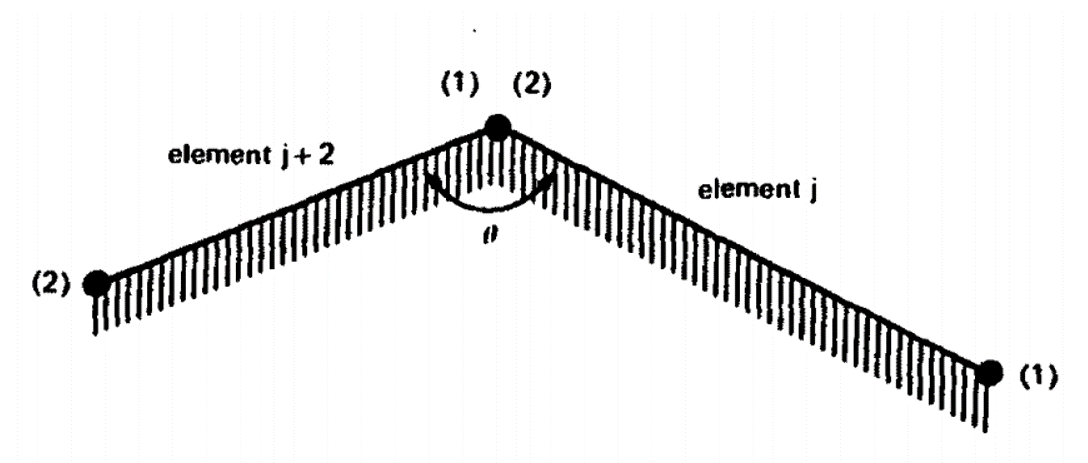
\includegraphics[scale=0.4]{Imagenes/nodos lineales continuos.png}
\caption{Intersección de elementos lineales continuos (Fuente:\cite{Brebbia})}\label{fig:Interseccion elementos continuos}
\end{figure}
\item \textbf{Definir el sistema de ecuaciones integrales a resolver.}\\
Operadores - Operators: Lo que en la ecuación \eqref{eq:Descripcion de matriz H y G} describimos como matrices $H$ y $G$, en esta plataforma son conocidos como operadores ('Single Layer Operator' y 'Double Layer Operator' respectivamente) y no son los únicos que están disponibles. Se definen de la siguiente forma:
\begin{equation}
\label{eq:Operadores de Laplace}
\begin{split}
V=\int_\Gamma g(x,y)d\Gamma\qquad & \textnormal{Single Layer Operator} \\
K=\int_\Gamma \frac{\delta g(x,y)}{\delta y}d\Gamma\qquad & \textnormal{Double Layer Operator} \\
K'=\int_\Gamma \frac{\delta g(x,y)}{\delta x}d\Gamma\qquad & \textnormal{Adjoint Double Layer Operator} \\
H=-\frac{\delta}{\delta x}\int_\Gamma \frac{\delta g(x,y)}{\delta y}d\Gamma\qquad & \textnormal{Hypersingular Boundary Operator} 
\end{split}
\end{equation}
Es importante destacar que es necesario precisar el modulo en el que serán ocupados: Laplace, Helmholtz o Helmholtz modificado. Existen otro operadores importantes como el operador de matriz identidad. La función $g(x,y)$ es la función de Green, la cual en todo este informe hemos definido como $u$.\\  
{Funciones de malla - Grid function: }Se trata de la función dominante, la función potencial en la frontera del elemento de estudio. También se utiliza para definir la condiciones de frontera de nuestro problema. En nuestro caso, las Grid function utilizadas fueron las condiciones de Neumann y Dirichlet indicadas en el problema.        
{Generación y resolución del sistema lineal: }Una vez que se tiene definido todo lo anterior se procede a definir el lado izquiero y derecho de la ecuación del problema, el cual posteriormente será resuelto usando $gmres$ al igual que el código anterior.
\item \textbf{Discretizar y resolver las ecuaciones.}\\
Ahora que ya calculamos el potencial y su derivada en los bordes es hora de calcular el comportamiento en su interior. Para eso haremos una matriz de vectores y 'anclaremos' en un punto en el eje $z$ para poder mostrar los resultados en un gráfico 2D al igual que en el código de Brebbia y Dominguez facilitando así la comparación de resultados.
Por útlimo se calculan los potenciales con las soluciones que obtuvimos en la parte anterior y se grafican.
\newpage
\end{enumerate}
\section{Planteamiento del problema.}\label{sec:Planteamiento del problema.}
\setcounter{figure}{0}
\setcounter{equation}{0}
La situación en la que nos enfrentamos en el problema es de una onda electromagnetica incidente en nuestro microhilo. Esta onda tiene un campo magnético incidente $B_i$ y un campo eléctrico incidente $E_i$. Denominaremos al volumen del micro-hilo como $\Omega_1$ y al volumen externo como $\Omega_2$ tal como se muestra en la figura \ref{fig:Representacion del problema}.
\begin{figure}[H]
\centering
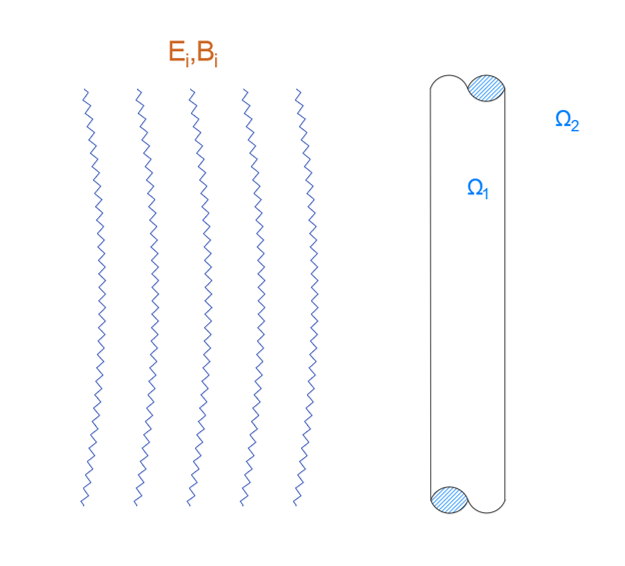
\includegraphics[width=12cm]{Imagenes/ondaincidente.png}
\caption{Situación del problema} \label{fig:Representacion del problema}
\end{figure}
Comenzaremos con las ecuaciones de Maxwell:
\begin{equation}
\begin{split}
&\nabla\cdot\textbf{D} = \rho\qquad\nabla\times\textbf{E} = -\frac{\partial\textbf{B}}{\partial t}\\
&\nabla\cdot\textbf{B} = 0\qquad\nabla\times\textbf{H} = J_f+\frac{\partial\textbf{D}}{\partial t}
\end{split}
\label{eq: Maxwell_inicial}
\end{equation}
Reescribiendo la ecuación \eqref{eq: Maxwell_inicial} en función solo de $B$ y $D$:
\begin{equation}
\begin{split}
&\nabla\cdot\textbf{D} = \rho\qquad \nabla\times\textbf{D} = -\varepsilon\frac{\partial\textbf{B}}{\partial t}\\
&\nabla\cdot\textbf{B} = 0\qquad\nabla\times\textbf{B} = \mu J_f+\mu\frac{\partial\textbf{D}}{\partial t}
\end{split}
\label{eq: Maxwell_soloBD}
\end{equation}
\newpage
Podemos suponer que una onda incidente en un entorno con propiedades electromagnéticas $\mu_2$ y $\varepsilon_2$ sufrirá de una perturbación si se encuentra con algún objeto con propiedades diferentes, tal como se plantea en nuestro problema.
\begin{figure}[H]
\centering
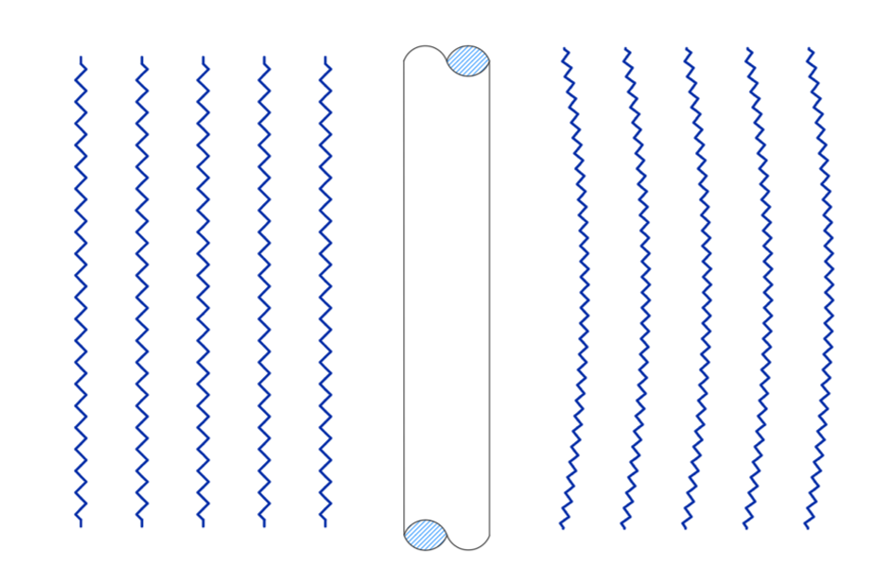
\includegraphics[width=16cm]{Imagenes/ondaincidente3.png}
\caption{Onda incidente perturbada.}\label{fig:Onda perturbada}
\end{figure}
Si ahora aplicamos las ecuaciones de Maxwell a la situación ilustrada en la figura \ref{fig:Onda perturbada}, obtenemos:
\begin{equation}
\label{eq:Onda perturbada}
\begin{split}
\left.
\begin{aligned}
&\nabla\cdot D_1 = \rho_1\qquad & \nabla\times D_1 = -\varepsilon_1\frac{\partial B_1}{\partial t}\\
&\nabla\cdot B_1 = 0\qquad & \nabla\times B_1 = \mu_1 J_{f1}+\mu_1\frac{\partial D_1}{\partial t}
\end{aligned}
\right\}
\quad\text{En }\Omega_1\\
\left.
\begin{aligned}
&\nabla\cdot D_2 = \rho_2\qquad & \nabla\times D_2 = -\varepsilon_2\frac{\partial B_2}{\partial t}\\
&\nabla\cdot B_2 = 0\qquad & \nabla\times B_2 = \mu_2 J_{f2}+\mu_2\frac{\partial D_2}{\partial t}
\end{aligned}
\right\}
\quad\text{En }\Omega_2\\
\left. 
D_1\cdot n=D_2\cdot n \qquad \frac{B_1}{\mu_1}\cdot n=\frac{B_2}{\mu_2}\cdot n
\right\}
\quad\text{En }\Gamma\\
\end{split}
\end{equation}
Debemos tener en cuenta que las propiedades del microhilo tendrán un efecto sobre el campo incidente. En caso de que las propiedades del volumen $\Omega_1$ sean iguales a los de $\Omega_2$, esto es $\varepsilon_1=\varepsilon_2$ y $\mu_1=\mu_2$\footnote{Por conveniencia matemática dejaremos todo escrito en términos del campo $\Omega_2$}. La situación descrita se puede ilustrar como en la imagen \ref{fig:Onda no afectada} y se puede representar en las ecuaciones de Maxwell de la forma:
\begin{equation}
\label{eq:Onda no afectada}
\begin{split}
\left.
\begin{aligned}
&\nabla\cdot D_i = \rho_1\qquad & \nabla\times D_1 = -\varepsilon_2\frac{\partial B_i}{\partial t}\\
&\nabla\cdot B_i = 0\qquad & \nabla\times B_i = \mu_2 J_{f1}+\mu_2\frac{\partial D_i}{\partial t}
\end{aligned}
\right\}
\quad\text{En }\Omega_1\\
\left.
\begin{aligned}
&\nabla\cdot D_i = \rho_2\qquad & \nabla\times D_i = -\varepsilon_2\frac{\partial B_i}{\partial t}\\
&\nabla\cdot B_i = 0\qquad & \nabla\times B_i = \mu_2 J_{f2}+\mu_2\frac{\partial D_i}{\partial t}
\end{aligned}
\right\}
\quad\text{En }\Omega_2\\
\left. 
D_i\cdot n=D_i\cdot n \qquad \frac{B_i}{\mu_2}\cdot n=\frac{B_i}{\mu_2}\cdot n
\right\}
\quad\text{En }\Gamma\\
\end{split}
\end{equation}
\begin{figure}[H]
\centering
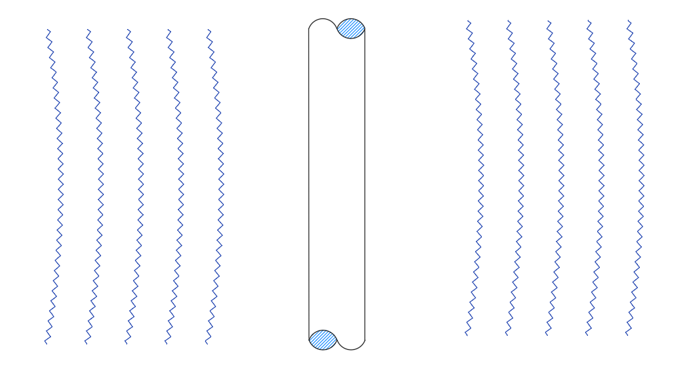
\includegraphics[width=16cm]{Imagenes/ondaincidente2.png}
\caption{Micro-hilo no tiene efecto sobre la onda.}\label{fig:Onda no afectada}
\end{figure}
Sabemos que en la situación expuesta en la ecuación \eqref{eq:Onda perturbada} el campo resultante, que es el expuesto en las ecuaciones puede verse como el campo incidente sumado al campo difundido producto del encuentro de la onda con al micro-hilo, por lo tanto los campos pueden ser representados como:
\begin{equation}
\label{eq:Descomposicion campos}
\begin{split}
D=D_i+D_d\\
B=B_i+B_d
\end{split}
\end{equation}
Donde $D_i$ y $B_i$ es el desplazamiento eléctrico inducido y $B_i$ es el campo magnético inducido.\\
Es correcto asumir que en nuestro sistema no hay corrientes electricas ni densidad de corriente por lo tanto los terminos de $\rho$ y $\vec{J}$ pueden ser eliminados. Por lo tanto podemos reescribir la ecuación \eqref{eq:Onda perturbada} como:
\begin{equation}
\label{eq:Onda perturbada y separada}
\begin{split}
\left.
\begin{aligned}
&\nabla\cdot D_{1d} + \nabla\cdot D_{i} = 0\qquad & \nabla\times D_{1d}+\nabla\times D_i = -\varepsilon_1\left(\frac{\partial B_{1d}}{\partial t}+\frac{\partial B_i}{\partial t}\right)\\
&\nabla\cdot B_{1d} +\nabla\cdot B_i = 0\qquad &  \nabla\times B_{1d}+\nabla\times B_i = \mu_1\left(\frac{\partial D_{1d}}{\partial t}+\frac{\partial D_i}{\partial t}\right)
\end{aligned}
\right\}
\quad\text{En }\Omega_1\\
\left.
\begin{aligned}
&\nabla\cdot D_{2d} + \nabla\cdot D_{i} = 0\qquad & \nabla\times D_{2d}+\nabla\times D_i = -\varepsilon_2\left(\frac{\partial B_{2d}}{\partial t}+\frac{\partial B_i}{\partial t}\right)\\
&\nabla\cdot B_{2d} +\nabla\cdot B_i = 0\qquad &  \nabla\times B_{2d}+\nabla\times B_i = \mu_2\left(\frac{\partial D_{2d}}{\partial t}+\frac{\partial D_i}{\partial t}\right)
\end{aligned}
\right\}
\quad\text{En }\Omega_2\\
\left. 
D_1\cdot n=D_2\cdot n \qquad \frac{B_1}{\mu_1}\cdot n=\frac{B_2}{\mu_2}\cdot n
\right\}
\quad\text{En }\Gamma\\
\end{split}
\end{equation}
Entonces si solo quisieramos saber como se comporta la onda difundida, solo es necesario restar la ecuación \eqref{eq:Onda no afectada} a la ecuación \eqref{eq:Onda perturbada y separada}:
\begin{equation}
\label{eq:Ondas restadas}
\begin{split}
\left.
\begin{aligned}
&\nabla\cdot D_{1d}= 0\qquad & \nabla\times D_{1d}= -\varepsilon_1\frac{\partial B_{1d}}{\partial t}-(\varepsilon_1-\varepsilon	_2)\frac{\partial B_i}{\partial t}\\
&\nabla\cdot B_{1d} = 0\qquad &  \nabla\times B_{1d}= \mu_1\frac{\partial D_{1d}}{\partial t}+(\mu_1-\mu_2)\frac{\partial D_i}{\partial t}
\end{aligned}
\right\}
\quad\text{En }\Omega_1\\
\left.
\begin{aligned}
&\nabla\cdot D_{1d}= 0\qquad & \nabla\times D_{1d}= -\varepsilon_1\frac{\partial B_{1d}}{\partial t}\\
&\nabla\cdot B_{1d} = 0\qquad &  \nabla\times B_{1d}= \mu_1\frac{\partial D_{1d}}{\partial t}
\end{aligned}
\right\}
\quad\text{En }\Omega_2\\
\left. 
D_{1d}\cdot n=D_{2d}\cdot n \qquad \left(\frac{1}{\mu_1}B_{1d}\cdot n-\frac{1}{\mu_2}B_{2d}\cdot n\right)=\left(\frac{1}{\mu_2}-\frac{1}{\mu_1}\right)B_i\cdot n
\right\}
\quad\text{En }\Gamma\\
\end{split}
\end{equation}
Se puede asumir una onda armónica con frecuencia $\omega$ para representar el desplazamiento eléctrico y el campo magnético:
$$B(x,t)=B(x)e^{i\omega t}$$
$$D(x,t)=D(x)e^{i\omega t}$$
La ecuación \eqref{eq:Ondas restadas} queda:
\begin{equation}
\label{eq:Ondas armonicas restadas }
\begin{split}
\left.
\begin{aligned}
&\nabla\cdot D_{1d}= 0\qquad & \nabla\times D_{1d}= -\varepsilon_1i\omega B_{1d}-(\varepsilon_1-\varepsilon	_2) i\omega B_i\\
&\nabla\cdot B_{1d} = 0\qquad &  \nabla\times B_{1d}= \mu_1 i\omega D_{1d}+(\mu_1-\mu_2)i\omega D_i
\end{aligned}
\right\}
\quad\text{En }\Omega_1\\
\left.
\begin{aligned}
&\nabla\cdot D_{1d}= 0\qquad & \nabla\times D_{1d}= -\varepsilon_1 i\omega B_{1d}\\
&\nabla\cdot B_{1d} = 0\qquad &  \nabla\times B_{1d}= \mu_1 i\omega D_{1d}
\end{aligned}
\right\}
\quad\text{En }\Omega_2\\
\left. 
D_{1d}\cdot n=D_{2d}\cdot n \qquad \left(\frac{1}{\mu_1}B_{1d}\cdot n-\frac{1}{\mu_2}B_{2d}\cdot n\right)=\left(\frac{1}{\mu_2}-\frac{1}{\mu_1}\right)B_i\cdot n
\right\}
\quad\text{En }\Gamma\\
\end{split}
\end{equation}
Podemos escribir las cantidades auxiliares:
\begin{equation}
\begin{gathered}
\begin{aligned}
b_i=\sqrt{\varepsilon_2}B_i &\qquad b_s=\sqrt{\varepsilon_2}B_s\\
d_i=\sqrt{\mu_2}D_i &\qquad d_s=\sqrt{\mu_2}D_s\\
x'=\frac{x}{d_x}
\end{aligned}
\end{gathered}
\end{equation}
A partir de esto podemos reescribir la ecuación \eqref{eq:Ondas armonicas restadas } utiliando las nuevas cantidades auxiliares:
\begin{equation}
\label{eq:Ondas armonicas restadas con cantidades auxiliares}
\begin{split}
\left.
\begin{aligned}
&\nabla\cdot d_{1d}= 0\qquad & \nabla\times d_{1d}= \frac{(\varepsilon_2-\varepsilon_1)}{\varepsilon_2} i\beta b_i-\frac{\varepsilon_1}{\varepsilon_2}i\beta b_{1d}\\
&\nabla\cdot b_{1d} = 0\qquad &  \nabla\times b_{1d}=\frac{(\mu_1-\mu_2)}{\mu_2}i\beta d_i \frac{\mu_1}{\mu_2}i\beta d_{1d}
\end{aligned}
\right\}
\quad\text{En }\Omega_1\\
\left.
\begin{aligned}
&\nabla\cdot d_{1d}= 0\qquad & \nabla\times d_{1d}= -i\beta b_{1d}\\
&\nabla\cdot b_{1d} = 0\qquad &  \nabla\times b_{1d}= i\beta d_{1d}
\end{aligned}
\right\}
\quad\text{En }\Omega_2\\
\left. 
d_{1d}\cdot n=d_{2d}\cdot n \qquad \left(\frac{1}{\mu_1}b_{1d}\cdot n-\frac{1}{\mu_2}b_{2d}\cdot n\right)=\left(\frac{1}{\mu_2}-\frac{1}{\mu_1}\right)b_i\cdot n
\right\}
\quad\text{En }\Gamma\\
\end{split}
\end{equation}
Con $\beta=wd\sqrt{\varepsilon_2\mu_2}$. Podemos expandir $d$ y $b$, utilizando $\beta$ como:
\begin{equation}
\begin{gathered}
d=d_s^{(0)}+\beta d_s^{(1)}+\beta^2 d_s^{(2)}...\\
b=b_s^{(0)}+\beta b_s^{(1)}+\beta^2 b_s^{(2)}...\\
\end{gathered}
\end{equation}
Y ahora considerando los términos de orden cero de la ecuación \eqref{eq:Ondas armonicas restadas con cantidades auxiliares}, escribimos solo los términos del campo mágnetico:
\begin{equation}
\label{eq:Sistema Campo Magnetico}
\begin{gathered}
\begin{aligned}
&\nabla\cdot b_{1d}^{(0)}= 0\qquad & \nabla\times b_{1d}^{(0)}= 0\\
&\nabla\cdot b_{2d}^{(0)} = 0\qquad &  \nabla\times b_{2d}^{(0)}= 0\\
\end{aligned}\\
\left(\frac{1}{\mu_1}b_{1d}^{(0)}\cdot n-\frac{1}{\mu_2}b_{2d}^{(0)}\cdot n\right)=\left(\frac{1}{\mu_2}-\frac{1}{\mu_1}\right)b_i\cdot n
%\quad\text{En }\Gamma
\end{gathered}
\end{equation}
Aplicando el operador $\nabla$ a las ecuaciones en $\Omega$ podemos concluir que:
\begin{itemize}
\item Por la identidad de la divergencia de un rotor:
\begin{equation*}
\begin{split}
\nabla \cdot (\nabla \times B_{1d}^{(0)})=0\\
\nabla \cdot (\nabla \times B_{2d}^{(0)})=0\\
\end{split}
\end{equation*}
Podemos determinar 	que los campos $B_{1d}$ y $B_{2d}$ son convervativos basandonos en que el rotor en ambos casos es cero, esto quiere decir que hay una función potencial que puede describir el comportamiento del campo.
\item Denominaremos como $\psi$ a la función escalar potencial que describirá nuestros campos:
$$\nabla \cdot \varphi = B_{d}$$
\item Nuevamente aplicamos el operador $\nabla$ pero esta vez en los gradientes del campo y utilizando la nueva notación con $\psi$, notar que estas ecuaciones se cumplen para el campo en $\Omega_1$ y $\Omega_2$ respectivamente:
$$\nabla^2\cdot \varphi_{1d}=0$$
$$\nabla^2\cdot \varphi_{2d}=0$$
\item Reescribimos las ecuaciones en el borde $\Gamma$ y añadimos una más:
$$\left(\frac{1}{\mu_1}\frac{\partial \varphi_{1d}}{\partial n}-\frac{1}{\mu_2}\frac{\partial \varphi_{2d}}{\partial n}\right)=\left(\frac{1}{\mu_2}-\frac{1}{\mu_1}\right)\frac{\partial \varphi_{i}}{\partial n}$$
$$\psi_{1d}=\varphi_{2d}\qquad\text{En la frontera }\Gamma$$
\end{itemize}
Finalmente nos encontramos con una ecuación diferencial con condiciones de borde, justamente lo necesario para resolver este problema utilizando el método de elementos de borde.

\begin{equation}
\label{eq:Ecuacion del problema}
\boxed{
\begin{gathered}
\nabla^2\cdot \varphi_{1d}=0,\qquad\nabla^2\cdot \varphi_{2d}=0\qquad\text{En }\Omega_1,\Omega_2\\
\left(\frac{1}{\mu_1}\frac{\partial \varphi_{1d}}{\partial n}-\frac{1}{\mu_2}\frac{\partial \varphi_{2d}}{\partial n}\right)=\left(\frac{1}{\mu_2}-\frac{1}{\mu_1}\right)\frac{\partial \varphi_{i}}{\partial n}\qquad\varphi_{1d}=\varphi_{2d}\qquad\text{En la frontera }\Gamma\\
\end{gathered}
}
\end{equation}
Y como se vio en la sección \ref{sec:BEM.} la ecuación \eqref{eq:Ecuacion del problema} puede representarse por una formulación de elementos de borde como:
\begin{equation}
\label{eq:Ecuacion con operadores sin condiciones}
\begin{gathered}
\frac{1}{2}\varphi_{1d}+K\cdot\varphi_{1d}-V\left(\frac{\partial}{\partial n}\varphi_{1d}\right)=0\\
\frac{1}{2}\varphi_{1d}-K\cdot\varphi_{1d}+V\left(\frac{\partial}{\partial n}\varphi_{2d}\right)=0\\
\text{En la frontera }\Gamma
\end{gathered}
\end{equation}
La primera ecuación presente en el conjunto mostrado en \eqref{eq:Ecuacion con operadores sin condiciones} es del mismo desarrollo que el mostrado en la sección citada. Sin embargo la segunda ecuación tiene los signos invertidos debido a que las normales apuntan en sentido contrario, $ergo$ los signos de los términos en donde las normales tienen incidencia deben tener distinto signo para que ambas tengan la misma convención de signos. Si además a lo anterior se aplican las condiciones de borde de \eqref{eq:Ecuacion del problema}:
\begin{equation}
\label{eq:Ecuacion de borde con condiciones de borde}
\begin{gathered}
\frac{1}{2}\varphi_{1d}+K\cdot\varphi_{1d}-V\left(\frac{\partial}{\partial n}\varphi_{1d}\right)=0\\
\frac{1}{2}\varphi_{2d}-K\cdot\varphi_{1d}+\mu_2 V\left(\frac{1}{\mu_1}\frac{\partial}{\partial n}\varphi_{2d}-\left(\frac{1}{\mu_2}-\frac{1}{\mu_1}\right)\frac{\partial}{\partial n}\varphi_{i}\right)=0\\
\text{En la frontera }\Gamma
\end{gathered}
\end{equation}
La forma matricial de la ecuación \eqref{eq:Ecuacion de borde con condiciones de borde} es:
\begin{equation}\label{eq:Forma matricial ecuacion 1}
\begin{bmatrix}
\frac{1}{2}I+K & -V \\ 
\frac{1}{2}I-K & \frac{\mu_2}{\mu_1}V
\end{bmatrix}
\begin{bmatrix}
\varphi_{1d}\\ 
\frac{\partial}{\partial n}\varphi_{1d}
\end{bmatrix}
=\begin{bmatrix}
0\\ 
\frac{\mu_1-\mu_2}{\mu_1}\frac{\partial \varphi_i}{\partial n}
\end{bmatrix}
\end{equation}
Donde $I$ sería la matriz identidad. Usando los mismos pasos matemáticos pero teniendo como 'campos iniciales' el campo eléctrico $E$ y la intensidad de campo magnético $H$ podemos llegar a una ecuación que tiene la misma estructura pero distintos coeficientes:
\begin{equation}
\begin{bmatrix}
\frac{1}{2}I+K & -V \\ 
\frac{1}{2}I-K & \frac{\varepsilon_1}{\varepsilon_2}V
\end{bmatrix}
\begin{bmatrix}
\varphi_{1d}\\ 
\frac{\partial}{\partial n}\varphi_{1d}
\end{bmatrix}
=\begin{bmatrix}
0\\ 
\frac{\varepsilon_2-\varepsilon_1}{\varepsilon_2}\frac{\partial \varphi_i}{\partial n}
\end{bmatrix}
\end{equation}
\subsection{Creación de mallas.}\label{sec:Creacion de mallas.}
Como se ha dicho en la sección \ref{sec:Biblioteca bempp.} es necesario una malla de estudio, a la cual aplicaremos las condiciones del problema. Corresponde utilizar el formato aceptado por la librería, $".msh"$. La creación de la geomtería de la malla se hace en el Software $SolidWorks$ en  donde se exporta el archivo en formato $STEP$:
\begin{figure}[H]
\centering
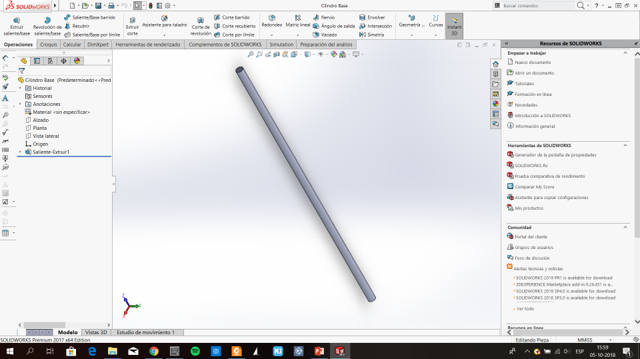
\includegraphics[scale=0.8]{Imagenes/Cilindro STEP.png}
\caption{Cilindro en SolidWorks}
\end{figure}
Luego, este archivo en formato $STEP$ se abre en el software $Gmsh$, el cual nos permitirá editar la forma de la malla, tamaño de los elementos, forma de los elementos, etc. Las mallas utilizadas tienen la forma de las imagenes que se muestran en \ref{fig:malla1}, \ref{fig:malla2} y \ref{fig:malla3}, cambiando el tamaño del elemento:
\begin{figure}[H]
\centering
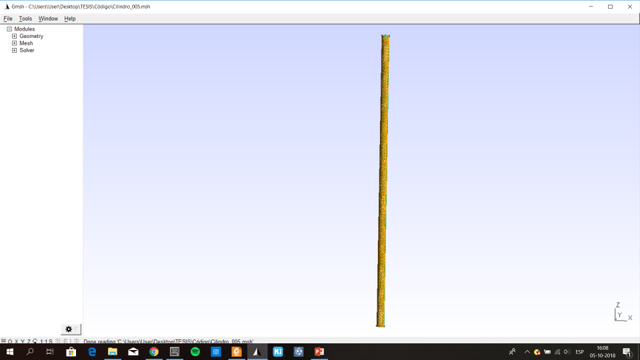
\includegraphics[scale=0.8]{Imagenes/malla1.png}
\caption{Malla vista completa}\label{fig:malla1}
\end{figure}
\begin{figure}[H]
\centering
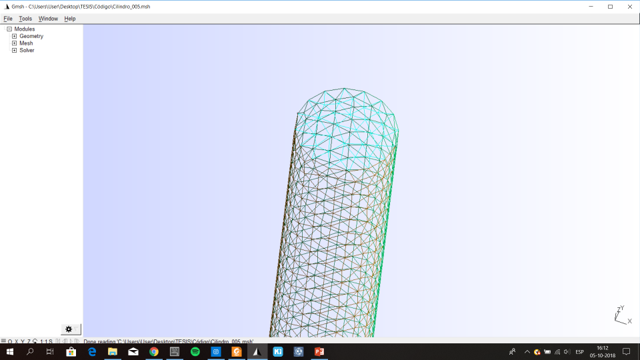
\includegraphics[scale=0.8]{Imagenes/malla2.png}
\caption{Malla detalle tapa}\label{fig:malla2}
\end{figure}
\begin{figure}[H]
\centering
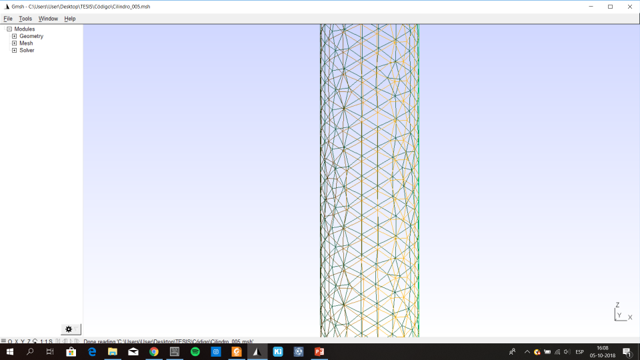
\includegraphics[scale=0.8]{Imagenes/malla3.png}
\caption{Malla detalle elementos}\label{fig:malla3}
\end{figure}
En el software $Gmsh$ también es posible verificar la dirección de los vectores normales y tangentes, por medio de inspección visual. Esto no es suficiente, por lo que abrimos la malla en $MeshLab$\cite{MeshLab} y verificamos no solo los puntos anteriores, sino también:
\begin{itemize}
\item Geometrías bien ubicadas.
\item Vectores normales en la dirección deseada.
\item Caras no duplicadas.
\end{itemize}
INSERTAR IMAGEN DE LA MALLA EN MESHLAB
\section{Desarrollo del problema.}
\setcounter{figure}{0}
\setcounter{equation}{0}
Como bien hablamos en capítulos anteriores, la resolución de la problematica planteada se realizará bajo la plataforma de $Jupyter\text{ }Notebook$. \\
Es importante partir comenzar importando librerías que serán necesarias para la resolución de los problemas, obviamente tenemos a $bempp$ y a $numpy$, una librería fundamental de python que contiene funciones de algebra lineal y arreglos de N-dimensiones que son utilizadas en todo método de resolución de ecuaciones diferenciales. Además de esto, se definen los nodos utilizados para realizar la cuadratura de Gauss.
\begin{tcolorbox}
\begin{Verbatim}[commandchars=\\\{\}]
\PY{c+c1}{\PYZsh{} Import libraries}
\PY{k+kn}{import} \PY{n+nn}{bempp}\PY{n+nn}{.}\PY{n+nn}{api}
\PY{k+kn}{import} \PY{n+nn}{numpy} \PY{k}{as} \PY{n+nn}{np}
\PY{n}{bempp}\PY{o}{.}\PY{n}{api}\PY{o}{.}\PY{n}{set\PYZus{}ipython\PYZus{}notebook\PYZus{}viewer}\PY{p}{(}\PY{p}{)}

\PY{c+c1}{\PYZsh{} Set quadrature options}        
\PY{n}{bempp}\PY{o}{.}\PY{n}{api}\PY{o}{.}\PY{n}{global\PYZus{}parameters}\PY{o}{.}\PY{n}{quadrature}\PY{o}{.}\PY{n}{near}\PY{o}{.}\PY{n}{double\PYZus{}order} \PY{o}{=} \PY{l+m+mi}{4}
\PY{n}{bempp}\PY{o}{.}\PY{n}{api}\PY{o}{.}\PY{n}{global\PYZus{}parameters}\PY{o}{.}\PY{n}{quadrature}\PY{o}{.}\PY{n}{medium}\PY{o}{.}\PY{n}{double\PYZus{}order} \PY{o}{=} \PY{l+m+mi}{4}
\PY{n}{bempp}\PY{o}{.}\PY{n}{api}\PY{o}{.}\PY{n}{global\PYZus{}parameters}\PY{o}{.}\PY{n}{quadrature}\PY{o}{.}\PY{n}{far}\PY{o}{.}\PY{n}{double\PYZus{}order} \PY{o}{=} \PY{l+m+mi}{4}
\end{Verbatim}
\end{tcolorbox}
Se define la malla, la cual es importada y creada como se explica en la subsección \ref{sec:Creacion de mallas.}. Se imprime la cantidad de elementos de la malla, lo que nos permitirá saber el tamaño de la matriz que resolveremos. Graficaremos la malla utilizando el comando $plot$, el cual grafica bajo la librería $plotly$, librería de gráficas de python y que nos permite revisar la gráfica de nuestra malla a mayor profundida. Sin embargo, por sus ajustes por defecto la malla puede verse algo rara, pero es solo un efecto óptico. 

\begin{tcolorbox}
\begin{Verbatim}[commandchars=\\\{\}]
\PY{c+c1}{\PYZsh{} Define grid}
\PY{n}{grid} \PY{o}{=} \PY{n}{bempp}\PY{o}{.}\PY{n}{api}\PY{o}{.}\PY{n}{import\PYZus{}grid}\PY{p}{(}\PY{l+s+s2}{\PYZdq{}}\PY{l+s+s2}{Cilindro\PYZus{}005.msh}\PY{l+s+s2}{\PYZdq{}}\PY{p}{)}

\PY{c+c1}{\PYZsh{} Print out the number of elements}
\PY{n}{number\PYZus{}of\PYZus{}elements} \PY{o}{=} \PY{n}{grid}\PY{o}{.}\PY{n}{leaf\PYZus{}view}\PY{o}{.}\PY{n}{entity\PYZus{}count}\PY{p}{(}\PY{l+m+mi}{0}\PY{p}{)}    
\PY{n+nb}{print}\PY{p}{(}\PY{l+s+s2}{\PYZdq{}}\PY{l+s+s2}{The grid has }\PY{l+s+si}{\PYZob{}0\PYZcb{}}\PY{l+s+s2}{ elements.}\PY{l+s+s2}{\PYZdq{}}\PY{o}{.}\PY{n}{format}\PY{p}{(}\PY{n}{number\PYZus{}of\PYZus{}elements}\PY{p}{)}\PY{p}{)}

\PY{c+c1}{\PYZsh{} Plot the grid}
\PY{n}{grid.plot()}
\end{Verbatim}
\end{tcolorbox}
\begin{figure}[H]
\centering
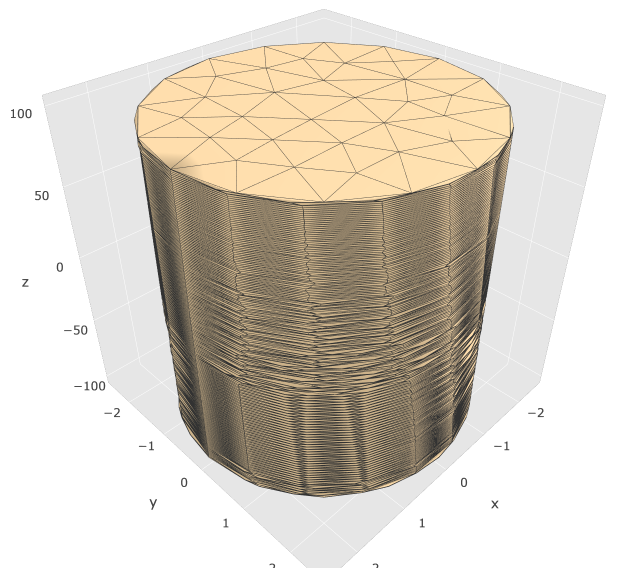
\includegraphics[scale=0.9]{Imagenes/graficas/Situacion 1/Malla/malla 1.png} 
\caption{Malla con ajustes predeterminados en $plotly$}
\end{figure}
\begin{figure}[H]
\centering
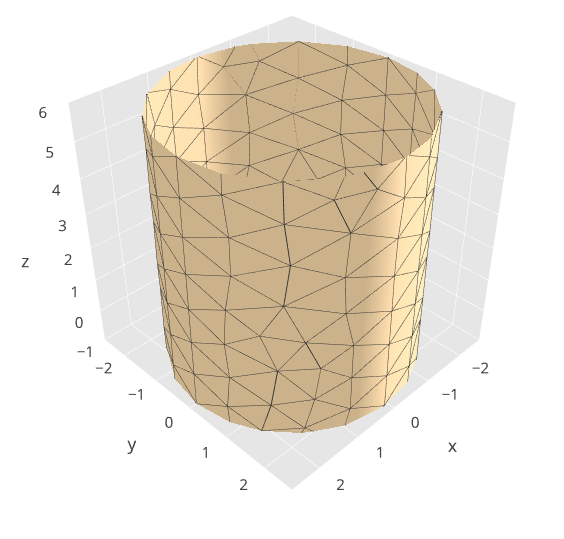
\includegraphics[scale=0.8]{Imagenes/graficas/Situacion 1/Malla/malla 2.png} 
\caption{Malla con eje $z$ no 'comprimido' en $plotly$}
\end{figure}
El siguiente paso a seguir es crear los espacios de funciones, en este caso se ha dejado como una variable el orden de los espacios. Se imprime el valor del grado de libertad del espacio. \\
Se ingresan los datos del problemas.
\begin{tcolorbox}
\begin{Verbatim}[commandchars=\\\{\}]
\PY{c+c1}{\PYZsh{} Set the Dirichlet and Neumann orders}
\PY{n}{order\PYZus{}neumann} \PY{o}{=} \PY{l+m+mi}{0}
\PY{n}{order\PYZus{}dirichlet} \PY{o}{=} \PY{l+m+mi}{0}
 
 \PY{c+c1}{\PYZsh{} Create function spaces}       
\PY{n}{global\PYZus{}neumann\PYZus{}space} \PY{o}{=} \PY{n}{bempp}\PY{o}{.}\PY{n}{api}\PY{o}{.}\PY{n}{function\PYZus{}space}\PY{p}{(}\PY{n}{grid}\PY{p}{,} \PY{l+s+s2}{\PYZdq{}}\PY{l+s+s2}{DP}\PY{l+s+s2}{\PYZdq{}}\PY{p}{,} \PY{n}{order\PYZus{}neumann}\PY{p}{)}
\PY{n}{global\PYZus{}dirichlet\PYZus{}space} \PY{o}{=} \PY{n}{bempp}\PY{o}{.}\PY{n}{api}\PY{o}{.}\PY{n}{function\PYZus{}space}\PY{p}{(}\PY{n}{grid}\PY{p}{,} \PY{l+s+s2}{\PYZdq{}}\PY{l+s+s2}{DP}\PY{l+s+s2}{\PYZdq{}}\PY{p}{,} \PY{n}{order\PYZus{}dirichlet}\PY{p}{)}   
\PY{n}{NS} \PY{o}{=} \PY{n}{global\PYZus{}neumann\PYZus{}space}
\PY{n}{DS} \PY{o}{=} \PY{n}{global\PYZus{}dirichlet\PYZus{}space}

\PY{c+c1}{\PYZsh{} Print out the degrees of freedom}        
\PY{n+nb}{print}\PY{p}{(}\PY{l+s+s2}{\PYZdq{}}\PY{l+s+s2}{BEM dofs: }\PY{l+s+si}{\PYZob{}0\PYZcb{}}\PY{l+s+s2}{\PYZdq{}}\PY{o}{.}\PY{n}{format}\PY{p}{(}\PY{n}{NS}\PY{o}{.}\PY{n}{global\PYZus{}dof\PYZus{}count}\PY{p}{)}\PY{p}{)}

\PY{c+c1}{\PYZsh{} Problem data}        
\PY{n}{ep1} \PY{o}{=} \PY{l+m+mi}{200}
\PY{n}{ep2} \PY{o}{=} \PY{l+m+mi}{8}
\PY{n}{k} \PY{o}{=} \PY{l+m+mf}{0.125}
\end{Verbatim}
\end{tcolorbox}
Se generan los operadores que están presentes en la ecuación \eqref{eq:Forma matricial ecuacion 1}. Es importantehacer notar que el comando $blocked$ genera una matriz capaz de almacenar operadores, este será el lado izquierdo de la ecuación.
\begin{tcolorbox}
\begin{Verbatim}[commandchars=\\\{\}]
\PY{c+c1}{\PYZsh{}Operators}
\PY{n}{slp} \PY{o}{=} \PY{n}{bempp}\PY{o}{.}\PY{n}{api}\PY{o}{.}\PY{n}{operators}\PY{o}{.}\PY{n}{boundary}\PY{o}{.}\PY{n}{laplace}\PY{o}{.}\PY{n}{single\PYZus{}layer}\PY{p}{(}\PY{n}{NS}\PY{p}{,}\PY{n}{DS}\PY{p}{,}\PY{n}{DS}\PY{p}{)}
\PY{n}{dlp} \PY{o}{=} \PY{n}{bempp}\PY{o}{.}\PY{n}{api}\PY{o}{.}\PY{n}{operators}\PY{o}{.}\PY{n}{boundary}\PY{o}{.}\PY{n}{laplace}\PY{o}{.}\PY{n}{double\PYZus{}layer}\PY{p}{(}\PY{n}{DS}\PY{p}{,}\PY{n}{DS}\PY{p}{,}\PY{n}{DS}\PY{p}{)}        
\PY{n+nb}{id} \PY{o}{=} \PY{n}{bempp}\PY{o}{.}\PY{n}{api}\PY{o}{.}\PY{n}{operators}\PY{o}{.}\PY{n}{boundary}\PY{o}{.}\PY{n}{sparse}\PY{o}{.}\PY{n}{identity}\PY{p}{(}\PY{n}{DS}\PY{p}{,}\PY{n}{DS}\PY{p}{,}\PY{n}{DS}\PY{p}{)}
                
\PY{c+c1}{\PYZsh{}Formation of the left hand side matrix}
\PY{n}{blocked} \PY{o}{=} \PY{n}{bempp}\PY{o}{.}\PY{n}{api}\PY{o}{.}\PY{n}{BlockedOperator}\PY{p}{(}\PY{l+m+mi}{2}\PY{p}{,} \PY{l+m+mi}{2}\PY{p}{)}
\PY{n}{blocked}\PY{p}{[}\PY{l+m+mi}{0}\PY{p}{,} \PY{l+m+mi}{0}\PY{p}{]} \PY{o}{=} \PY{l+m+mf}{0.5} \PY{o}{*} \PY{n+nb}{id} \PY{o}{+} \PY{n}{dlp}
\PY{n}{blocked}\PY{p}{[}\PY{l+m+mi}{0}\PY{p}{,} \PY{l+m+mi}{1}\PY{p}{]} \PY{o}{=} \PY{o}{\PYZhy{}}\PY{n}{slp}
\PY{n}{blocked}\PY{p}{[}\PY{l+m+mi}{1}\PY{p}{,} \PY{l+m+mi}{0}\PY{p}{]} \PY{o}{=} \PY{l+m+mf}{0.5} \PY{o}{*} \PY{n+nb}{id} \PY{o}{\PYZhy{}} \PY{n}{dlp}
\PY{n}{blocked}\PY{p}{[}\PY{l+m+mi}{1}\PY{p}{,} \PY{l+m+mi}{1}\PY{p}{]} \PY{o}{=} \PY{n}{ep1}\PY{o}{/}\PY{n}{ep2} \PY{o}{*} \PY{n}{slp}
\end{Verbatim}
\end{tcolorbox}
El lado derecho de la ecuación está definido como una concatenación de dos funciones, que en el caso de la ecuación \eqref{eq:Forma matricial ecuacion 1} estás funciones son $0$ y $\frac{\partial \varphi_i}{\partial n}$, al definir $\varphi=e^{jkx}$ se puede representar su derivada en la normal como se presenta a continuación. Además estás funciones, recordemos, viven en un espacio de funciones que hemos definido más arriba, por lo que se debe definir la función dentro del espacio correspondiente para generar la 'función de malla':
\begin{tcolorbox}
\begin{Verbatim}[commandchars=\\\{\}]
\PY{c+c1}{\PYZsh{}Definition of functions}
\PY{k}{def} \PY{n+nf}{funcion1}\PY{p}{(}\PY{n}{x}\PY{p}{,} \PY{n}{n}\PY{p}{,} \PY{n}{domain\PYZus{}index}\PY{p}{,} \PY{n}{result}\PY{p}{)}\PY{p}{:}
\PY{n}{result}\PY{p}{[}\PY{p}{:}\PY{p}{]} \PY{o}{=} \PY{p}{(}\PY{p}{(}\PY{n}{ep2} \PY{o}{\PYZhy{}} \PY{n}{ep1}\PY{p}{)} \PY{o}{/} \PY{n}{ep2}\PY{p}{)} \PY{o}{*} \PY{p}{(}\PY{l+m+mf}{1.} \PY{o}{*} \PY{l+m+mi}{1}\PY{n}{j} \PY{o}{*} \PY{n}{k} \PY{o}{*} \PY{n}{n}\PY{p}{[}\PY{l+m+mi}{0}\PY{p}{]} \PY{o}{*} \PY{n}{np}\PY{o}{.}\PY{n}{exp}\PY{p}{(}\PY{l+m+mi}{1}\PY{n}{j} \PY{o}{*} \PY{n}{k} \PY{o}{*} \PY{n}{x}\PY{p}{[}\PY{l+m+mi}{0}\PY{p}{]}\PY{p}{)}\PY{p}{)}
        
\PY{k}{def} \PY{n+nf}{cero}\PY{p}{(}\PY{n}{x}\PY{p}{,} \PY{n}{n}\PY{p}{,} \PY{n}{domain\PYZus{}index}\PY{p}{,} \PY{n}{result}\PY{p}{)}\PY{p}{:}
\PY{n}{result}\PY{p}{[}\PY{p}{:}\PY{p}{]} \PY{o}{=} \PY{l+m+mi}{0}

\PY{c+c1}{\PYZsh{}Formation functions in the space}            
\PY{n}{funcion\PYZus{}fun} \PY{o}{=} \PY{n}{bempp}\PY{o}{.}\PY{n}{api}\PY{o}{.}\PY{n}{GridFunction}\PY{p}{(}\PY{n}{DS}\PY{p}{,} \PY{n}{fun}\PY{o}{=}\PY{n}{funcion1}\PY{p}{)}        
\PY{n}{cero\PYZus{}fun} \PY{o}{=} \PY{n}{bempp}\PY{o}{.}\PY{n}{api}\PY{o}{.}\PY{n}{GridFunction}\PY{p}{(}\PY{n}{NS}\PY{p}{,} \PY{n}{fun}\PY{o}{=}\PY{n}{cero}\PY{p}{)}
\end{Verbatim}
\end{tcolorbox}
Para resolver el sistema de ecuaciones existen varias formas de hacerlo, con distinta rapidez, precisión, entre otros factores. En la mayoría podemos ver como converge la solución, la cantidad de iteraciones realizadas para llegar a esta y la precisión de la misma, que en este caso viene dedo por el ajuste $tol$. La discretización de ambos lados de la ecuación viene por el comando $use\_strong\_form$, lo cual puede relizarse separadamente, pero aumenta la cantidad de capacidad computacional necesaria.
\begin{tcolorbox}
\begin{Verbatim}[commandchars=\\\{\}]
\PY{c+c1}{\PYZsh{}Solving the matrix system}
\PY{n}{sol}\PY{p}{,} \PY{n}{info}\PY{p}{,} \PY{n}{it\PYZus{}count} \PY{o}{=} \PY{n}{bempp}\PY{o}{.}\PY{n}{api}\PY{o}{.}\PY{n}{linalg}\PY{o}{.}\PY{n}{gmres}\PY{p}{(}\PY{n}{blocked}\PY{p}{,} \PY{p}{[}\PY{n}{cero\PYZus{}fun}\PY{p}{,} \PY{n}{funcion\PYZus{}fun}\PY{p}{]}\PY{p}{,}
		\PY{n}{use\PYZus{}strong\PYZus{}form}\PY{o}{=}\PY{k+kc}{True}\PY{p}{,} \PY{n}{return\PYZus{}iteration\PYZus{}count}\PY{o}{=}\PY{k+kc}{True}\PY{p}{,} \PY{n}{tol}\PY{o}{=}\PY{l+m+mf}{1e\PYZhy{}3}\PY{p}{)}

\PY{c+c1}{\PYZsh{}Print number of iterations}         
\PY{n+nb}{print}\PY{p}{(}\PY{l+s+s2}{\PYZdq{}}\PY{l+s+s2}{The linear system was solved in }\PY{l+s+si}{\PYZob{}0\PYZcb{}}\PY{l+s+s2}{ iterations}\PY{l+s+s2}{\PYZdq{}}\PY{o}{.}\PY{n}{format}\PY{p}{(}\PY{n}{it\PYZus{}count}\PY{p}{)}\PY{p}{)}
\end{Verbatim}
\end{tcolorbox}
Cuando se resuelve el sistema de matrices, se obtiene '2' soluciones. Como vemos en la ecuación \eqref{eq:Forma matricial ecuacion 1} obtenemos $\varphi_1$ y $\frac{\partial \varphi_1}{\partial n}$, lo que visto en el código serían la $solution\_dirichl$ y $solution\_neumann$ respectivamente. Como nos interesa ver la forma de la onda disipada, graficamos esta onda, es decir, $solution\_dirichl$ en torno a nuestra malla de estudio.
\begin{tcolorbox}
\begin{Verbatim}[commandchars=\\\{\}]
\PY{c+c1}{\PYZsh{}Divide the solution} 
\PY{n}{solution\PYZus{}dirichl}\PY{p}{,} \PY{n}{solution\PYZus{}neumann} \PY{o}{=} \PY{n}{sol}

\PY{c+c1}{\PYZsh{}Plot the solution} 
\PY{n}{solution\PYZus{}dirichl}\PY{o}{.}\PY{n}{plot}\PY{p}{(}\PY{p}{)}
\end{Verbatim}
\end{tcolorbox}
\begin{figure}[H]
\centering
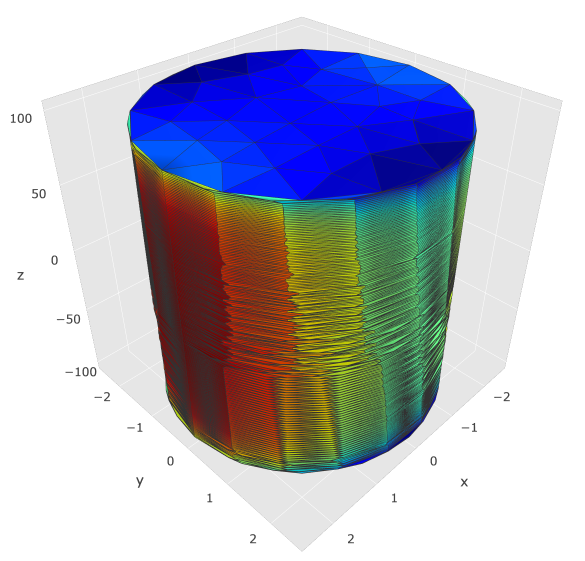
\includegraphics[width=16cm]{Imagenes/graficas/Situacion 1/Solucion ecuacion 1/3d.png}
\caption{Solución situacion 1}
\end{figure}

Además de ver la solución en 3D, se hace necesario ver en detalle que sucede el centro  de nuestra malla, por lo que generar una malla 2D sobre un plano $z$ determinado nos ayudaría a ver el comportamiento de la onda dentro de, en este caso, el cable.
\begin{tcolorbox}
\begin{Verbatim}[commandchars=\\\{\}]
\PY{c+c1}{\PYZsh{}Generate the grid} 
\PY{n}{n\PYZus{}grid\PYZus{}points} \PY{o}{=} \PY{l+m+mi}{200}
\PY{n}{xmin}\PY{p}{,} \PY{n}{xmax}\PY{p}{,} \PY{n}{ymin}\PY{p}{,} \PY{n}{ymax}\PY{o}{=}\PY{p}{[}\PY{o}{\PYZhy{}}\PY{l+m+mi}{3}\PY{p}{,}\PY{l+m+mi}{3}\PY{p}{,}\PY{o}{\PYZhy{}}\PY{l+m+mi}{3}\PY{p}{,}\PY{l+m+mi}{3}\PY{p}{]}
\PY{n}{plot\PYZus{}grid} \PY{o}{=} \PY{n}{np}\PY{o}{.}\PY{n}{mgrid}\PY{p}{[}\PY{n}{xmin}\PY{p}{:}\PY{n}{xmax}\PY{p}{:}\PY{n}{n\PYZus{}grid\PYZus{}points}\PY{o}{*}\PY{l+m+mi}{1}\PY{n}{j}\PY{p}{,}\PY{n}{ymin}\PY{p}{:}\PY{n}{ymax}\PY{p}{:}\PY{n}{n\PYZus{}grid\PYZus{}points}\PY{o}{*}\PY{l+m+mi}{1}\PY{n}{j}\PY{p}{]}
\PY{n}{points} \PY{o}{=} \PY{n}{np}\PY{o}{.}\PY{n}{vstack}\PY{p}{(}\PY{p}{(}\PY{n}{plot\PYZus{}grid}\PY{p}{[}\PY{l+m+mi}{0}\PY{p}{]}\PY{o}{.}\PY{n}{ravel}\PY{p}{(}\PY{p}{)}\PY{p}{,}
         \PY{n}{plot\PYZus{}grid}\PY{p}{[}\PY{l+m+mi}{1}\PY{p}{]}\PY{o}{.}\PY{n}{ravel}\PY{p}{(}\PY{p}{)}\PY{p}{,}
	 \PY{n}{np}\PY{o}{.}\PY{n}{zeros}\PY{p}{(}\PY{n}{plot\PYZus{}grid}\PY{p}{[}\PY{l+m+mi}{0}\PY{p}{]}\PY{o}{.}\PY{n}{size}\PY{p}{)}\PY{p}{)}\PY{p}{)}
\end{Verbatim}
\end{tcolorbox}

Se crean las funciones de espacio utilizando la malla en 3D.
\begin{tcolorbox}
\begin{Verbatim}[commandchars=\\\{\}]
\PY{c+c1}{\PYZsh{}Generate the spaces} 
\PY{n}{dp0\PYZus{}space} \PY{o}{=} \PY{n}{bempp}\PY{o}{.}\PY{n}{api}\PY{o}{.}\PY{n}{function\PYZus{}space}\PY{p}{(}\PY{n}{grid}\PY{p}{,} \PY{l+s+s2}{\PYZdq{}}\PY{l+s+s2}{DP}\PY{l+s+s2}{\PYZdq{}}\PY{p}{,} \PY{l+m+mi}{0}\PY{p}{)}
\PY{n}{p1\PYZus{}space} \PY{o}{=} \PY{n}{bempp}\PY{o}{.}\PY{n}{api}\PY{o}{.}\PY{n}{function\PYZus{}space}\PY{p}{(}\PY{n}{grid}\PY{p}{,} \PY{l+s+s2}{\PYZdq{}}\PY{l+s+s2}{DP}\PY{l+s+s2}{\PYZdq{}}\PY{p}{,} \PY{l+m+mi}{0}\PY{p}{)}
\end{Verbatim}
\end{tcolorbox}

Se generan los operadores bajo los puntos especificados en la malla 2D, es decir bajo un plano $z$ especificado.
\begin{tcolorbox}
\begin{Verbatim}[commandchars=\\\{\}]
\PY{c+c1}{\PYZsh{}Generate the operators} 
\PY{n}{slp\PYZus{}pot} \PY{o}{=} \PY{n}{bempp}\PY{o}{.}\PY{n}{api}\PY{o}{.}\PY{n}{operators}\PY{o}{.}\PY{n}{potential}\PY{o}{.}\PY{n}{laplace}\PY{o}{.}\PY{n}{single\PYZus{}layer}\PY{p}{(}\PY{n}{dp0\PYZus{}space}\PY{p}{,} \PY{n}{points}\PY{p}{)}
\PY{n}{dlp\PYZus{}pot} \PY{o}{=} \PY{n}{bempp}\PY{o}{.}\PY{n}{api}\PY{o}{.}\PY{n}{operators}\PY{o}{.}\PY{n}{potential}\PY{o}{.}\PY{n}{laplace}\PY{o}{.}\PY{n}{double\PYZus{}layer}\PY{p}{(}\PY{n}{p1\PYZus{}space}\PY{p}{,} \PY{n}{points}\PY{p}{)}
\end{Verbatim}
\end{tcolorbox}

Se evalua la solución en todos los puntos del plano, que vienen siendo los puntos internos de la malla en un plano especifico, es decir, se utiliza la ecuación \eqref{eq:Calculo puntos internos discretizada}.
\begin{tcolorbox}
\begin{Verbatim}[commandchars=\\\{\}]
\PY{c+c1}{\PYZsh{}Evaluation in internal points} 
\PY{n}{u\PYZus{}evaluated} \PY{o}{=} \PY{n}{slp\PYZus{}pot} \PY{o}{*} \PY{n}{solution\PYZus{}neumann} \PY{o}{\PYZhy{}} \PY{n}{dlp\PYZus{}pot} \PY{o}{*} \PY{n}{solution\PYZus{}dirichl}
\end{Verbatim}
\end{tcolorbox}
Finalmente se grafica la solución obtenida, en este caso obtendremos una solución con una parte imaginaria, a nosotros para graficar solo nos interesa la parte real de la solución por lo que filtraremos bajo este criterio. Otro criterio de filtro es que los resultados fuera de la malla, son irrelevantes, por lo que se eliminan. |
\begin{tcolorbox}
\begin{Verbatim}[commandchars=\\\{\}]
\PY{c+c1}{\PYZsh{} The next command ensures that plots are shown within the IPython notebook}
\PY{o}{\PYZpc{}}\PY{k}{matplotlib} inline                
\PY{k+kn}{from} \PY{n+nn}{matplotlib} \PY{k}{import} \PY{n}{pylab} \PY{k}{as} \PY{n}{plt}
         
\PY{c+c1}{\PYZsh{}Plot the results}       
\PY{n}{fig}\PY{p}{,}\PY{n}{ax} \PY{o}{=} \PY{n}{plt}\PY{o}{.}\PY{n}{subplots}\PY{p}{(}\PY{p}{)}
\PY{n}{ax}\PY{o}{.}\PY{n}{scatter}\PY{p}{(}\PY{n}{u\PYZus{}evaluated}\PY{o}{.}\PY{n}{real}\PY{p}{,}\PY{n}{u\PYZus{}evaluated}\PY{o}{.}\PY{n}{imag}\PY{p}{)}
\PY{c+c1}{\PYZsh{} Filter out solution values that are associated} 
\PY{c+c1}{\PYZsh{} with points outside the unit circle.}
\PY{n}{u\PYZus{}evaluated} \PY{o}{=} \PY{p}{(}\PY{n}{u\PYZus{}evaluated}\PY{p}{)}\PY{o}{.}\PY{n}{reshape}\PY{p}{(}\PY{p}{(}\PY{n}{n\PYZus{}grid\PYZus{}points}\PY{p}{,}\PY{n}{n\PYZus{}grid\PYZus{}points}\PY{p}{)}\PY{p}{)}
\PY{n}{radius} \PY{o}{=} \PY{n}{np}\PY{o}{.}\PY{n}{sqrt}\PY{p}{(}\PY{n}{plot\PYZus{}grid}\PY{p}{[}\PY{l+m+mi}{0}\PY{p}{]}\PY{o}{*}\PY{o}{*}\PY{l+m+mi}{2} \PY{o}{+} \PY{n}{plot\PYZus{}grid}\PY{p}{[}\PY{l+m+mi}{1}\PY{p}{]}\PY{o}{*}\PY{o}{*}\PY{l+m+mi}{2}\PY{p}{)}
\PY{n}{u\PYZus{}evaluated}\PY{p}{[}\PY{n}{radius}\PY{o}{\PYZgt{}}\PY{l+m+mi}{2}\PY{p}{]} \PY{o}{=} \PY{n}{np}\PY{o}{.}\PY{n}{nan}
\PY{n}{fig} \PY{o}{=} \PY{n}{plt}\PY{o}{.}\PY{n}{figure}\PY{p}{(}\PY{n}{figsize}\PY{o}{=}\PY{p}{(}\PY{l+m+mi}{10}\PY{p}{,} \PY{l+m+mi}{8}\PY{p}{)}\PY{p}{)}
\PY{n}{plt}\PY{o}{.}\PY{n}{imshow}\PY{p}{(}\PY{p}{(}\PY{p}{(}\PY{n}{u\PYZus{}evaluated}\PY{o}{.}\PY{n}{real}\PY{p}{)}\PY{p}{)}\PY{p}{,} \PY{n}{extent}\PY{o}{=}\PY{p}{(}\PY{o}{\PYZhy{}}\PY{l+m+mi}{3}\PY{p}{,}\PY{l+m+mi}{3}\PY{p}{,}\PY{o}{\PYZhy{}}\PY{l+m+mi}{3}\PY{p}{,}\PY{l+m+mi}{3}\PY{p}{)}\PY{p}{)}
\PY{n}{plt}\PY{o}{.}\PY{n}{title}\PY{p}{(}\PY{l+s+s1}{\PYZsq{}}\PY{l+s+s1}{Computed solution}\PY{l+s+s1}{\PYZsq{}}\PY{p}{)}
\PY{n}{plt}\PY{o}{.}\PY{n}{colorbar}\PY{p}{(}\PY{p}{)}
\end{Verbatim}
\end{tcolorbox}
\begin{figure}[H]
\centering
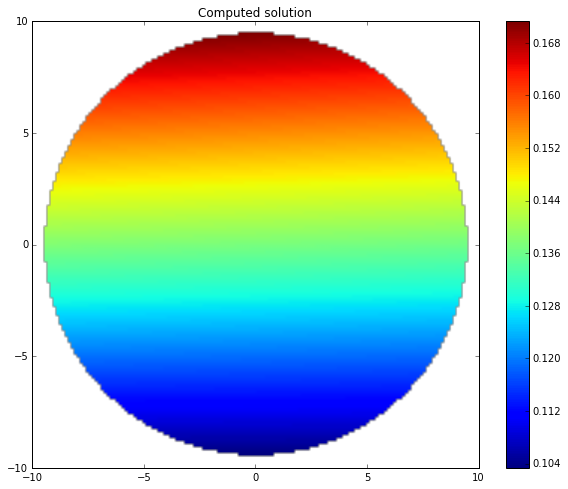
\includegraphics[width=10cm]{Imagenes/graficas/Situacion 1/Solucion ecuacion 1/2d.png}
\caption{Solución situacion 1}
\end{figure}

\begin{tcolorbox}
\begin{Verbatim}[commandchars=\\\{\}]
\PY{c+c1}{\PYZsh{}Preambulo}
\PY{k+kn}{import} \PY{n+nn}{numpy} \PY{k}{as} \PY{n+nn}{np}
\PY{k+kn}{import} \PY{n+nn}{bempp}\PY{n+nn}{.}\PY{n+nn}{api}
\PY{n}{omega} \PY{o}{=} \PY{l+m+mf}{2.}\PY{o}{*}\PY{n}{np}\PY{o}{.}\PY{n}{pi}\PY{o}{*}\PY{l+m+mf}{10.e9}
\PY{n}{e0} \PY{o}{=} \PY{l+m+mf}{8.854}\PY{o}{*}\PY{l+m+mf}{1e\PYZhy{}12}\PY{o}{*}\PY{l+m+mf}{1e\PYZhy{}18}
\PY{n}{mu0} \PY{o}{=} \PY{l+m+mf}{4.}\PY{o}{*}\PY{n}{np}\PY{o}{.}\PY{n}{pi}\PY{o}{*}\PY{l+m+mf}{1e\PYZhy{}7}\PY{o}{*}\PY{l+m+mf}{1e6}
\PY{n}{mue} \PY{o}{=} \PY{p}{(}\PY{l+m+mf}{1.}\PY{p}{)}\PY{o}{*}\PY{n}{mu0}
\PY{n}{ee} \PY{o}{=} \PY{p}{(}\PY{l+m+mf}{16.}\PY{p}{)}\PY{o}{*}\PY{n}{e0}
\PY{n}{mui} \PY{o}{=} \PY{p}{(}\PY{o}{\PYZhy{}}\PY{l+m+mf}{2.9214}\PY{o}{+}\PY{l+m+mf}{0.5895}\PY{n}{j}\PY{p}{)}\PY{o}{*}\PY{n}{mu0}
\PY{n}{ei} \PY{o}{=} \PY{p}{(}\PY{l+m+mf}{82629.2677}\PY{o}{\PYZhy{}}\PY{l+m+mf}{200138.2211}\PY{n}{j}\PY{p}{)}\PY{o}{*}\PY{n}{e0}
\PY{n}{k} \PY{o}{=} \PY{n}{omega}\PY{o}{*}\PY{n}{np}\PY{o}{.}\PY{n}{sqrt}\PY{p}{(}\PY{n}{e0}\PY{o}{*}\PY{n}{mu0}\PY{p}{)}
\PY{n}{lam} \PY{o}{=} \PY{l+m+mi}{2}\PY{o}{*}\PY{n}{np}\PY{o}{.}\PY{n}{pi}\PY{o}{/}\PY{n}{k}
\PY{n}{nm} \PY{o}{=} \PY{n}{np}\PY{o}{.}\PY{n}{sqrt}\PY{p}{(}\PY{p}{(}\PY{n}{ee}\PY{o}{*}\PY{n}{mue}\PY{p}{)}\PY{o}{/}\PY{p}{(}\PY{n}{e0}\PY{o}{*}\PY{n}{mu0}\PY{p}{)}\PY{p}{)}
\PY{n}{nc} \PY{o}{=} \PY{n}{np}\PY{o}{.}\PY{n}{sqrt}\PY{p}{(}\PY{p}{(}\PY{n}{ei}\PY{o}{*}\PY{n}{mui}\PY{p}{)}\PY{o}{/}\PY{p}{(}\PY{n}{e0}\PY{o}{*}\PY{n}{mu0}\PY{p}{)}\PY{p}{)}
\PY{n}{alfa\PYZus{}m} \PY{o}{=} \PY{n}{mue}\PY{o}{/}\PY{n}{mu0}
\PY{n}{alfa\PYZus{}c} \PY{o}{=} \PY{n}{mui}\PY{o}{/}\PY{n}{mue}
\PY{n}{antena} \PY{o}{=} \PY{n}{np}\PY{o}{.}\PY{n}{array}\PY{p}{(}\PY{p}{[}\PY{p}{[}\PY{l+m+mf}{1e4}\PY{p}{]}\PY{p}{,}\PY{p}{[}\PY{l+m+mf}{0.}\PY{p}{]}\PY{p}{,}\PY{p}{[}\PY{l+m+mf}{0.}\PY{p}{]}\PY{p}{]}\PY{p}{)}
\PY{n+nb}{print}\PY{p}{(}\PY{l+s+s2}{\PYZdq{}}\PY{l+s+s2}{Numero de onda exterior:}\PY{l+s+s2}{\PYZdq{}}\PY{p}{,} \PY{n}{k}\PY{p}{)}
\PY{n+nb}{print}\PY{p}{(}\PY{l+s+s2}{\PYZdq{}}\PY{l+s+s2}{Indice de refraccion matriz:}\PY{l+s+s2}{\PYZdq{}}\PY{p}{,} \PY{n}{nm}\PY{p}{)}
\PY{n+nb}{print}\PY{p}{(}\PY{l+s+s2}{\PYZdq{}}\PY{l+s+s2}{Indice de refraccion conductor:}\PY{l+s+s2}{\PYZdq{}}\PY{p}{,} \PY{n}{nc}\PY{p}{)}
\PY{n+nb}{print}\PY{p}{(}\PY{l+s+s2}{\PYZdq{}}\PY{l+s+s2}{Numero de onda interior matriz:}\PY{l+s+s2}{\PYZdq{}}\PY{p}{,} \PY{n}{nm}\PY{o}{*}\PY{n}{k}\PY{p}{)}
\PY{n+nb}{print}\PY{p}{(}\PY{l+s+s2}{\PYZdq{}}\PY{l+s+s2}{Numero de onda interior conductor:}\PY{l+s+s2}{\PYZdq{}}\PY{p}{,} \PY{n}{nm}\PY{o}{*}\PY{n}{nc}\PY{o}{*}\PY{n}{k}\PY{p}{)}
\PY{n+nb}{print}\PY{p}{(}\PY{l+s+s2}{\PYZdq{}}\PY{l+s+s2}{Indice de transmision matriz:}\PY{l+s+s2}{\PYZdq{}}\PY{p}{,} \PY{n}{alfa\PYZus{}m}\PY{p}{)}
\PY{n+nb}{print}\PY{p}{(}\PY{l+s+s2}{\PYZdq{}}\PY{l+s+s2}{Indice de transmision conductor:}\PY{l+s+s2}{\PYZdq{}}\PY{p}{,} \PY{n}{alfa\PYZus{}c}\PY{p}{)}
\PY{n+nb}{print}\PY{p}{(}\PY{l+s+s2}{\PYZdq{}}\PY{l+s+s2}{Longitud de onda:}\PY{l+s+s2}{\PYZdq{}}\PY{p}{,} \PY{n}{lam}\PY{p}{,} \PY{l+s+s2}{\PYZdq{}}\PY{l+s+s2}{micras}\PY{l+s+s2}{\PYZdq{}}\PY{p}{)}
\end{Verbatim}
\end{tcolorbox}


\begin{tcolorbox}
\begin{Verbatim}[commandchars=\\\{\}]
\PY{c+c1}{\PYZsh{}Importando mallas}
\PY{n}{grid\PYZus{}0} \PY{o}{=} \PY{n}{bempp}\PY{o}{.}\PY{n}{api}\PY{o}{.}\PY{n}{import\PYZus{}grid}\PY{p}{(}\PY{l+s+s2}{\PYZdq{}}\PY{l+s+s2}{Cilindro\PYZus{}005.msh}\PY{l+s+s2}{\PYZdq{}}\PY{p}{)}
\end{Verbatim}
\end{tcolorbox}

\begin{tcolorbox}
\begin{Verbatim}[commandchars=\\\{\}]
\PY{c+c1}{\PYZsh{}Funciones de dirichlet y neumann}
\PY{k}{def} \PY{n+nf}{dirichlet\PYZus{}fun}\PY{p}{(}\PY{n}{x}\PY{p}{,} \PY{n}{n}\PY{p}{,} \PY{n}{domain\PYZus{}index}\PY{p}{,} \PY{n}{result}\PY{p}{)}\PY{p}{:}
\PY{n}{result}\PY{p}{[}\PY{l+m+mi}{0}\PY{p}{]} \PY{o}{=} \PY{l+m+mf}{1.} \PY{o}{*} \PY{n}{np}\PY{o}{.}\PY{n}{exp}\PY{p}{(}\PY{l+m+mi}{1}\PY{n}{j} \PY{o}{*} \PY{n}{k} \PY{o}{*} \PY{n}{x}\PY{p}{[}\PY{l+m+mi}{0}\PY{p}{]}\PY{p}{)}
\PY{k}{def} \PY{n+nf}{neumann\PYZus{}fun}\PY{p}{(}\PY{n}{x}\PY{p}{,} \PY{n}{n}\PY{p}{,} \PY{n}{domain\PYZus{}index}\PY{p}{,} \PY{n}{result}\PY{p}{)}\PY{p}{:}
\PY{n}{result}\PY{p}{[}\PY{l+m+mi}{0}\PY{p}{]} \PY{o}{=} \PY{l+m+mf}{1.} \PY{o}{*} \PY{l+m+mi}{1}\PY{n}{j} \PY{o}{*} \PY{n}{k} \PY{o}{*} \PY{n}{n}\PY{p}{[}\PY{l+m+mi}{0}\PY{p}{]} \PY{o}{*} \PY{n}{np}\PY{o}{.}\PY{n}{exp}\PY{p}{(}\PY{l+m+mi}{1}\PY{n}{j} \PY{o}{*} \PY{n}{k} \PY{o}{*} \PY{n}{x}\PY{p}{[}\PY{l+m+mi}{0}\PY{p}{]}\PY{p}{)}
\end{Verbatim}
\end{tcolorbox}


\begin{tcolorbox}
\begin{Verbatim}[commandchars=\\\{\}]
\PY{c+c1}{\PYZsh{}Operadores multitrazo}
\PY{n}{Ai\PYZus{}0} \PY{o}{=} \PY{n}{bempp}\PY{o}{.}\PY{n}{api}\PY{o}{.}\PY{n}{operators}\PY{o}{.}\PY{n}{boundary}\PY{o}{.}\PY{n}{helmholtz}\PY{o}{.}\PY{n}{multitrace\PYZus{}operator}\PY{p}{(}\PY{n}{grid\PYZus{}0}\PY{p}{,} \PY{n}{nm} \PY{o}{*} \PY{n}{nc} \PY{o}{*} \PY{n}{k}\PY{p}{)}
\PY{n}{Ae\PYZus{}0} \PY{o}{=} \PY{n}{bempp}\PY{o}{.}\PY{n}{api}\PY{o}{.}\PY{n}{operators}\PY{o}{.}\PY{n}{boundary}\PY{o}{.}\PY{n}{helmholtz}\PY{o}{.}\PY{n}{multitrace\PYZus{}operator}\PY{p}{(}\PY{n}{grid\PYZus{}0}\PY{p}{,} \PY{n}{nm} \PY{o}{*} \PY{n}{k}\PY{p}{)}
         
\PY{c+c1}{\PYZsh{}Transmision en Multitrazo}
\PY{n}{Ai\PYZus{}0}\PY{p}{[}\PY{l+m+mi}{0}\PY{p}{,}\PY{l+m+mi}{1}\PY{p}{]} \PY{o}{=} \PY{n}{Ai\PYZus{}0}\PY{p}{[}\PY{l+m+mi}{0}\PY{p}{,}\PY{l+m+mi}{1}\PY{p}{]}\PY{o}{*}\PY{n}{alfa\PYZus{}c}
\PY{n}{Ai\PYZus{}0}\PY{p}{[}\PY{l+m+mi}{1}\PY{p}{,}\PY{l+m+mi}{1}\PY{p}{]} \PY{o}{=} \PY{n}{Ai\PYZus{}0}\PY{p}{[}\PY{l+m+mi}{1}\PY{p}{,}\PY{l+m+mi}{1}\PY{p}{]}\PY{o}{*}\PY{n}{alfa\PYZus{}c}
         
\PY{c+c1}{\PYZsh{}Acople interior y exterior}
\PY{n}{op\PYZus{}0} \PY{o}{=} \PY{p}{(}\PY{n}{Ai\PYZus{}0} \PY{o}{+} \PY{n}{Ae\PYZus{}0}\PY{p}{)}
\end{Verbatim}
\end{tcolorbox}


\begin{tcolorbox}
\begin{Verbatim}[commandchars=\\\{\}]
\PY{c+c1}{\PYZsh{}Espacios}
\PY{n}{dirichlet\PYZus{}space\PYZus{}0} \PY{o}{=} \PY{n}{Ai\PYZus{}0}\PY{p}{[}\PY{l+m+mi}{0}\PY{p}{,}\PY{l+m+mi}{0}\PY{p}{]}\PY{o}{.}\PY{n}{domain}
\PY{n}{neumann\PYZus{}space\PYZus{}0} \PY{o}{=} \PY{n}{Ai\PYZus{}0}\PY{p}{[}\PY{l+m+mi}{0}\PY{p}{,}\PY{l+m+mi}{1}\PY{p}{]}\PY{o}{.}\PY{n}{domain}
\end{Verbatim}
\end{tcolorbox}

\begin{tcolorbox}
\begin{Verbatim}[commandchars=\\\{\}]
\PY{c+c1}{\PYZsh{}Operadores identidad}
\PY{n}{ident\PYZus{}0} \PY{o}{=} \PY{n}{bempp}\PY{o}{.}\PY{n}{api}\PY{o}{.}\PY{n}{operators}\PY{o}{.}\PY{n}{boundary}\PY{o}{.}\PY{n}{sparse}\PY{o}{.}\PY{n}{identity}\PY{p}{(}\PY{n}{neumann\PYZus{}space\PYZus{}0}\PY{p}{,} \PY{n}{neumann\PYZus{}space\PYZus{}0}\PY{p}{,} \PY{n}{neumann\PYZus{}space\PYZus{}0}\PY{p}{)}
\end{Verbatim}
\end{tcolorbox}


\begin{tcolorbox}
\begin{Verbatim}[commandchars=\\\{\}]
\PY{c+c1}{\PYZsh{}Matriz de operadores}
\PY{n}{blocked} \PY{o}{=} \PY{n}{bempp}\PY{o}{.}\PY{n}{api}\PY{o}{.}\PY{n}{BlockedOperator}\PY{p}{(}\PY{l+m+mi}{2}\PY{p}{,}\PY{l+m+mi}{2}\PY{p}{)}
\end{Verbatim}
\end{tcolorbox}


\begin{tcolorbox}
\begin{Verbatim}[commandchars=\\\{\}]
{\color{incolor}In [{\color{incolor}27}]:} \PY{c+c1}{\PYZsh{}Diagonal}
\PY{n}{blocked}\PY{p}{[}\PY{l+m+mi}{0}\PY{p}{,}\PY{l+m+mi}{0}\PY{p}{]} \PY{o}{=} \PY{n}{op\PYZus{}0}\PY{p}{[}\PY{l+m+mi}{0}\PY{p}{,}\PY{l+m+mi}{0}\PY{p}{]}
\PY{n}{blocked}\PY{p}{[}\PY{l+m+mi}{0}\PY{p}{,}\PY{l+m+mi}{1}\PY{p}{]} \PY{o}{=} \PY{n}{op\PYZus{}0}\PY{p}{[}\PY{l+m+mi}{0}\PY{p}{,}\PY{l+m+mi}{1}\PY{p}{]}
\PY{n}{blocked}\PY{p}{[}\PY{l+m+mi}{1}\PY{p}{,}\PY{l+m+mi}{0}\PY{p}{]} \PY{o}{=} \PY{n}{op\PYZus{}0}\PY{p}{[}\PY{l+m+mi}{1}\PY{p}{,}\PY{l+m+mi}{0}\PY{p}{]}
\PY{n}{blocked}\PY{p}{[}\PY{l+m+mi}{1}\PY{p}{,}\PY{l+m+mi}{1}\PY{p}{]} \PY{o}{=} \PY{n}{op\PYZus{}0}\PY{p}{[}\PY{l+m+mi}{1}\PY{p}{,}\PY{l+m+mi}{1}\PY{p}{]}
\PY{n}{blocked}\PY{p}{[}\PY{l+m+mi}{1}\PY{p}{,}\PY{l+m+mi}{1}\PY{p}{]} \PY{o}{=} \PY{n}{blocked}\PY{p}{[}\PY{l+m+mi}{1}\PY{p}{,}\PY{l+m+mi}{1}\PY{p}{]} \PY{o}{+} \PY{l+m+mf}{0.5} \PY{o}{*} \PY{n}{ident\PYZus{}0} \PY{o}{*} \PY{p}{(}\PY{n}{alfa\PYZus{}c} \PY{o}{\PYZhy{}} \PY{l+m+mi}{1}\PY{p}{)}
\end{Verbatim}
\end{tcolorbox}


\begin{tcolorbox}
\begin{Verbatim}[commandchars=\\\{\}]
\PY{c+c1}{\PYZsh{}Condiciones de borde}
\PY{n}{dirichlet\PYZus{}grid\PYZus{}fun\PYZus{}0} \PY{o}{=} \PY{n}{bempp}\PY{o}{.}\PY{n}{api}\PY{o}{.}\PY{n}{GridFunction}\PY{p}{(}\PY{n}{dirichlet\PYZus{}space\PYZus{}0}\PY{p}{,} \PY{n}{fun}\PY{o}{=}\PY{n}{dirichlet\PYZus{}fun}\PY{p}{)}
\PY{n}{neumann\PYZus{}grid\PYZus{}fun\PYZus{}0} \PY{o}{=} \PY{n}{bempp}\PY{o}{.}\PY{n}{api}\PY{o}{.}\PY{n}{GridFunction}\PY{p}{(}\PY{n}{neumann\PYZus{}space\PYZus{}0}\PY{p}{,} \PY{n}{fun}\PY{o}{=}\PY{n}{neumann\PYZus{}fun}\PY{p}{)}
         
\PY{c+c1}{\PYZsh{}Discretizacion lado derecho}
\PY{n}{rhs} \PY{o}{=} \PY{n}{np}\PY{o}{.}\PY{n}{concatenate}\PY{p}{(}\PY{p}{[}\PY{n}{dirichlet\PYZus{}grid\PYZus{}fun\PYZus{}0}\PY{o}{.}\PY{n}{coefficients}\PY{p}{,} \PY{n}{neumann\PYZus{}grid\PYZus{}fun\PYZus{}0}\PY{o}{.}\PY{n}{coefficients}\PY{p}{]}\PY{p}{)}
\end{Verbatim}
\end{tcolorbox}

\begin{tcolorbox}
\begin{Verbatim}[commandchars=\\\{\}]
\PY{c+c1}{\PYZsh{}Discretizacion lado izquierdo}
\PY{n}{blocked\PYZus{}discretizado} \PY{o}{=} \PY{n}{blocked}\PY{o}{.}\PY{n}{strong\PYZus{}form}\PY{p}{(}\PY{p}{)}
\end{Verbatim}
\end{tcolorbox}


\begin{tcolorbox}
\begin{Verbatim}[commandchars=\\\{\}]
\PY{c+c1}{\PYZsh{}Sistema de ecuaciones}
\PY{k+kn}{import} \PY{n+nn}{inspect}
\PY{k+kn}{from} \PY{n+nn}{scipy}\PY{n+nn}{.}\PY{n+nn}{sparse}\PY{n+nn}{.}\PY{n+nn}{linalg} \PY{k}{import} \PY{n}{gmres}
\PY{n}{array\PYZus{}it} \PY{o}{=} \PY{n}{np}\PY{o}{.}\PY{n}{array}\PY{p}{(}\PY{p}{[}\PY{p}{]}\PY{p}{)}
\PY{n}{array\PYZus{}frame} \PY{o}{=} \PY{n}{np}\PY{o}{.}\PY{n}{array}\PY{p}{(}\PY{p}{[}\PY{p}{]}\PY{p}{)}
\PY{n}{it\PYZus{}count} \PY{o}{=} \PY{l+m+mi}{0}
\PY{k}{def} \PY{n+nf}{iteration\PYZus{}counter}\PY{p}{(}\PY{n}{x}\PY{p}{)}\PY{p}{:}
	\PY{k}{global} \PY{n}{array\PYZus{}it}
	\PY{k}{global} \PY{n}{array\PYZus{}frame}
	\PY{k}{global} \PY{n}{it\PYZus{}count}
	\PY{n}{it\PYZus{}count} \PY{o}{+}\PY{o}{=} \PY{l+m+mi}{1}
	\PY{n}{frame} \PY{o}{=} \PY{n}{inspect}\PY{o}{.}\PY{n}{currentframe}\PY{p}{(}\PY{p}{)}\PY{o}{.}\PY{n}{f\PYZus{}back}
	\PY{n}{array\PYZus{}it} \PY{o}{=} \PY{n}{np}\PY{o}{.}\PY{n}{append}\PY{p}{(}\PY{n}{array\PYZus{}it}\PY{p}{,} \PY{n}{it\PYZus{}count}\PY{p}{)}
	\PY{n}{array\PYZus{}frame} \PY{o}{=} \PY{n}{np}\PY{o}{.}\PY{n}{append}\PY{p}{(}\PY{n}{array\PYZus{}frame}\PY{p}{,} \PY{n}{frame}\PY{o}{.}\PY{n}{f\PYZus{}locals}\PY{p}{[}\PY{l+s+s2}{\PYZdq{}}\PY{l+s+s2}{resid}\PY{l+s+s2}{\PYZdq{}}\PY{p}{]}\PY{p}{)}
	\PY{n+nb}{print} \PY{n}{it\PYZus{}count}\PY{p}{,} \PY{n}{frame}\PY{o}{.}\PY{n}{f\PYZus{}locals}\PY{p}{[}\PY{l+s+s2}{\PYZdq{}}\PY{l+s+s2}{resid}\PY{l+s+s2}{\PYZdq{}}\PY{p}{]}
\PY{n+nb}{print}\PY{p}{(}\PY{l+s+s2}{\PYZdq{}}\PY{l+s+s2}{Shape of matrix: }\PY{l+s+si}{\PYZob{}0\PYZcb{}}\PY{l+s+s2}{\PYZdq{}}\PY{o}{.}\PY{n}{format}\PY{p}{(}\PY{n}{blocked\PYZus{}discretizado}\PY{o}{.}\PY{n}{shape}\PY{p}{)}\PY{p}{)}
\PY{n}{x}\PY{p}{,}\PY{n}{info} \PY{o}{=} \PY{n}{gmres}\PY{p}{(}\PY{n}{blocked\PYZus{}discretizado}\PY{p}{,} \PY{n}{rhs}\PY{p}{,} \PY{n}{tol}\PY{o}{=}\PY{l+m+mf}{1e\PYZhy{}5}\PY{p}{,} \PY{n}{callback} \PY{o}{=} \PY{n}{iteration\PYZus{}counter}\PY{p}{,} \PY{n}{maxiter} \PY{o}{=} \PY{l+m+mi}{50000}\PY{p}{)}
\PY{n+nb}{print}\PY{p}{(}\PY{l+s+s2}{\PYZdq{}}\PY{l+s+s2}{El sistema fue resuelto en }\PY{l+s+si}{\PYZob{}0\PYZcb{}}\PY{l+s+s2}{ iteraciones}\PY{l+s+s2}{\PYZdq{}}\PY{o}{.}\PY{n}{format}\PY{p}{(}\PY{n}{it\PYZus{}count}\PY{p}{)}\PY{p}{)}
\PY{n}{np}\PY{o}{.}\PY{n}{savetxt}\PY{p}{(}\PY{l+s+s2}{\PYZdq{}}\PY{l+s+s2}{Solucion.out}\PY{l+s+s2}{\PYZdq{}}\PY{p}{,} \PY{n}{x}\PY{p}{,} \PY{n}{delimiter}\PY{o}{=}\PY{l+s+s2}{\PYZdq{}}\PY{l+s+s2}{,}\PY{l+s+s2}{\PYZdq{}}\PY{p}{)}
\end{Verbatim}
\end{tcolorbox}


\begin{tcolorbox}
\begin{Verbatim}[commandchars=\\\{\}]
{\color{incolor}In [{\color{incolor} }]:} \PY{c+c1}{\PYZsh{}Campo interior}
\PY{n}{interior\PYZus{}field\PYZus{}dirichlet\PYZus{}m} \PY{o}{=} \PY{n}{bempp}\PY{o}{.}\PY{n}{api}\PY{o}{.}\PY{n}{GridFunction}\PY{p}{(}\PY{n}{dirichlet\PYZus{}space\PYZus{}m}\PY{p}{,} \PY{n}{coefficients}\PY{o}{=}\PY{n}{x}\PY{p}{[}\PY{p}{:}\PY{n}{dirichlet\PYZus{}space\PYZus{}m}\PY{o}{.}\PY{n}{global\PYZus{}dof\PYZus{}count}\PY{p}{]}\PY{p}{)}
\PY{n}{interior\PYZus{}field\PYZus{}neumann\PYZus{}m} \PY{o}{=} \PY{n}{bempp}\PY{o}{.}\PY{n}{api}\PY{o}{.}\PY{n}{GridFunction}\PY{p}{(}\PY{n}{neumann\PYZus{}space\PYZus{}m}\PY{p}{,}\PY{n}{coefficients}\PY{o}{=}\PY{n}{x}\PY{p}{[}\PY{n}{dirichlet\PYZus{}space\PYZus{}m}\PY{o}{.}\PY{n}{global\PYZus{}dof\PYZus{}count}\PY{p}{:}\PY{n}{dirichlet\PYZus{}space\PYZus{}m}\PY{o}{.}\PY{n}{global\PYZus{}dof\PYZus{}count} \PY{o}{+} \PY{n}{neumann\PYZus{}space\PYZus{}m}\PY{o}{.}\PY{n}{global\PYZus{}dof\PYZus{}count}\PY{p}{]}\PY{p}{)}
        
\PY{c+c1}{\PYZsh{}Campo exterior}
\PY{n}{exterior\PYZus{}field\PYZus{}dirichlet\PYZus{}m} \PY{o}{=} \PY{n}{interior\PYZus{}field\PYZus{}dirichlet\PYZus{}m}
\PY{n}{exterior\PYZus{}field\PYZus{}neumann\PYZus{}m} \PY{o}{=} \PY{n}{interior\PYZus{}field\PYZus{}neumann\PYZus{}m}\PY{o}{*}\PY{p}{(}\PY{l+m+mf}{1.}\PY{o}{/}\PY{n}{alfa\PYZus{}m}\PY{p}{)}
        
\PY{c+c1}{\PYZsh{}Calculo campo en antena}
\PY{n}{slp\PYZus{}pot\PYZus{}ext\PYZus{}m} \PY{o}{=} \PY{n}{bempp}\PY{o}{.}\PY{n}{api}\PY{o}{.}\PY{n}{operators}\PY{o}{.}\PY{n}{potential}\PY{o}{.}\PY{n}{helmholtz}\PY{o}{.}\PY{n}{single\PYZus{}layer}\PY{p}{(}\PY{n}{dirichlet\PYZus{}space\PYZus{}m}\PY{p}{,} \PY{n}{antena}\PY{p}{,} \PY{n}{k}\PY{p}{)}
\PY{n}{dlp\PYZus{}pot\PYZus{}ext\PYZus{}m} \PY{o}{=} \PY{n}{bempp}\PY{o}{.}\PY{n}{api}\PY{o}{.}\PY{n}{operators}\PY{o}{.}\PY{n}{potential}\PY{o}{.}\PY{n}{helmholtz}\PY{o}{.}\PY{n}{double\PYZus{}layer}\PY{p}{(}\PY{n}{dirichlet\PYZus{}space\PYZus{}m}\PY{p}{,} \PY{n}{antena}\PY{p}{,} \PY{n}{k}\PY{p}{)}
\PY{n}{Campo\PYZus{}en\PYZus{}antena} \PY{o}{=} \PY{p}{(}\PY{n}{dlp\PYZus{}pot\PYZus{}ext\PYZus{}m} \PY{o}{*} \PY{n}{exterior\PYZus{}field\PYZus{}dirichlet\PYZus{}m} \PY{o}{\PYZhy{}} \PY{n}{slp\PYZus{}pot\PYZus{}ext\PYZus{}m} \PY{o}{*} \PY{n}{exterior\PYZus{}field\PYZus{}neumann\PYZus{}m}\PY{p}{)}\PY{o}{.}\PY{n}{ravel}\PY{p}{(}\PY{p}{)} \PY{o}{+} \PY{n}{np}\PY{o}{.}\PY{n}{exp}\PY{p}{(}\PY{l+m+mi}{1}\PY{n}{j}\PY{o}{*}\PY{n}{k}\PY{o}{*}\PY{n}{antena}\PY{p}{[}\PY{l+m+mi}{0}\PY{p}{]}\PY{p}{)}
\PY{n+nb}{print} \PY{l+s+s2}{\PYZdq{}}\PY{l+s+s2}{Valor del campo en receptor:}\PY{l+s+s2}{\PYZdq{}}\PY{p}{,} \PY{n}{Campo\PYZus{}en\PYZus{}antena}
\end{Verbatim}
\end{tcolorbox}


\begin{tcolorbox}

\end{tcolorbox}


\begin{tcolorbox}

\end{tcolorbox}

\begin{tcolorbox}

\end{tcolorbox}


\begin{tcolorbox}

\end{tcolorbox}


\begin{tcolorbox}

\end{tcolorbox}


\begin{tcolorbox}

\end{tcolorbox}


\begin{tcolorbox}

\end{tcolorbox}
\newpage
\section{Bibliografía.}
\begin{thebibliography}{9}
\bibitem{Wikipedia}
  Leslie Lamport,
  \textit{\LaTeX: a document preparation system},
  Addison Wesley, Massachusetts,
  2nd edition,
  1994.
\bibitem{Brebbia} \textsc{C.A. Brebbia.} y \textsc{J. Dominguez},\textit{ Boundary elements, an introduction course}, Second Edition, Chapter 1 y 2, 1992.
\bibitem{bempp} \textsc{bempp services},\textit{ https://bempp.com/}
\bibitem{camposvectoriales} \textsc{Universidad Nacional de La Plata – Facultad de Ciencias Exactas},\textit{Guía 6 - Campos vectoriales}, ANALISIS MATEMATICO II, 2014
\bibitem{camposvectoriales2} \textsc{Universidad Almería},\textit{Guía 'Tema 9 - Campos escalates y campos vectoriales. Integrales de línea y superficia'}
\bibitem{Solvingbempp}
\textit{Smigaj, W., Betcke, T., Arridge, S., Phillips, J., and Schweiger}, M. 2012. \textsc{Solving boundary integral problems
with BEM++.} ACM Trans. Math. Softw. V, N, Article A (January YYYY), 50 pages.
\bibitem{MeshLab} \textit{P. Cignoni, M. Callieri, M. Corsini, M. Dellepiane, F. Ganovelli, G. Ranzuglia} \textsc{MeshLab: an Open-Source Mesh Processing Tool} Sixth Eurographics Italian Chapter Conference, page 129-136, 2008
\bibitem{Gmsh} \textit{C. Geuzaine and J.-F. Remacle.} \textsc{Gmsh: a three-dimensional finite element mesh generator with built-in pre- and post-processing facilities.} International Journal for Numerical Methods in Engineering 79(11), pp. 1309-1331, 2009.

\end{thebibliography}
\end{document}
